\documentclass[crop=false,class=book,oneside]{standalone}
%----------------------------Preamble-------------------------------%
%---------------------------Packages----------------------------%
\usepackage{geometry}
\geometry{b5paper, margin=1.0in}
\usepackage[T1]{fontenc}
\usepackage{graphicx, float}            % Graphics/Images.
\usepackage{natbib}                     % For bibliographies.
\bibliographystyle{agsm}                % Bibliography style.
\usepackage[french, english]{babel}     % Language typesetting.
\usepackage[dvipsnames]{xcolor}         % Color names.
\usepackage{listings}                   % Verbatim-Like Tools.
\usepackage{mathtools, esint, mathrsfs} % amsmath and integrals.
\usepackage{amsthm, amsfonts, amssymb}  % Fonts and theorems.
\usepackage{tcolorbox}                  % Frames around theorems.
\usepackage{upgreek}                    % Non-Italic Greek.
\usepackage{fmtcount, etoolbox}         % For the \book{} command.
\usepackage[newparttoc]{titlesec}       % Formatting chapter, etc.
\usepackage{titletoc}                   % Allows \book in toc.
\usepackage[nottoc]{tocbibind}          % Bibliography in toc.
\usepackage[titles]{tocloft}            % ToC formatting.
\usepackage{pgfplots, tikz}             % Drawing/graphing tools.
\usepackage{imakeidx}                   % Used for index.
\usetikzlibrary{
    calc,                   % Calculating right angles and more.
    angles,                 % Drawing angles within triangles.
    arrows.meta,            % Latex and Stealth arrows.
    quotes,                 % Adding labels to angles.
    positioning,            % Relative positioning of nodes.
    decorations.markings,   % Adding arrows in the middle of a line.
    patterns,
    arrows
}                                       % Libraries for tikz.
\pgfplotsset{compat=1.9}                % Version of pgfplots.
\usepackage[font=scriptsize,
            labelformat=simple,
            labelsep=colon]{subcaption} % Subfigure captions.
\usepackage[font={scriptsize},
            hypcap=true,
            labelsep=colon]{caption}    % Figure captions.
\usepackage[pdftex,
            pdfauthor={Ryan Maguire},
            pdftitle={Mathematics and Physics},
            pdfsubject={Mathematics, Physics, Science},
            pdfkeywords={Mathematics, Physics, Computer Science, Biology},
            pdfproducer={LaTeX},
            pdfcreator={pdflatex}]{hyperref}
\hypersetup{
    colorlinks=true,
    linkcolor=blue,
    filecolor=magenta,
    urlcolor=Cerulean,
    citecolor=SkyBlue
}                           % Colors for hyperref.
\usepackage[toc,acronym,nogroupskip,nopostdot]{glossaries}
\usepackage{glossary-mcols}
%------------------------Theorem Styles-------------------------%
\theoremstyle{plain}
\newtheorem{theorem}{Theorem}[section]

% Define theorem style for default spacing and normal font.
\newtheoremstyle{normal}
    {\topsep}               % Amount of space above the theorem.
    {\topsep}               % Amount of space below the theorem.
    {}                      % Font used for body of theorem.
    {}                      % Measure of space to indent.
    {\bfseries}             % Font of the header of the theorem.
    {}                      % Punctuation between head and body.
    {.5em}                  % Space after theorem head.
    {}

% Italic header environment.
\newtheoremstyle{thmit}{\topsep}{\topsep}{}{}{\itshape}{}{0.5em}{}

% Define environments with italic headers.
\theoremstyle{thmit}
\newtheorem*{solution}{Solution}

% Define default environments.
\theoremstyle{normal}
\newtheorem{example}{Example}[section]
\newtheorem{definition}{Definition}[section]
\newtheorem{problem}{Problem}[section]

% Define framed environment.
\tcbuselibrary{most}
\newtcbtheorem[use counter*=theorem]{ftheorem}{Theorem}{%
    before=\par\vspace{2ex},
    boxsep=0.5\topsep,
    after=\par\vspace{2ex},
    colback=green!5,
    colframe=green!35!black,
    fonttitle=\bfseries\upshape%
}{thm}

\newtcbtheorem[auto counter, number within=section]{faxiom}{Axiom}{%
    before=\par\vspace{2ex},
    boxsep=0.5\topsep,
    after=\par\vspace{2ex},
    colback=Apricot!5,
    colframe=Apricot!35!black,
    fonttitle=\bfseries\upshape%
}{ax}

\newtcbtheorem[use counter*=definition]{fdefinition}{Definition}{%
    before=\par\vspace{2ex},
    boxsep=0.5\topsep,
    after=\par\vspace{2ex},
    colback=blue!5!white,
    colframe=blue!75!black,
    fonttitle=\bfseries\upshape%
}{def}

\newtcbtheorem[use counter*=example]{fexample}{Example}{%
    before=\par\vspace{2ex},
    boxsep=0.5\topsep,
    after=\par\vspace{2ex},
    colback=red!5!white,
    colframe=red!75!black,
    fonttitle=\bfseries\upshape%
}{ex}

\newtcbtheorem[auto counter, number within=section]{fnotation}{Notation}{%
    before=\par\vspace{2ex},
    boxsep=0.5\topsep,
    after=\par\vspace{2ex},
    colback=SeaGreen!5!white,
    colframe=SeaGreen!75!black,
    fonttitle=\bfseries\upshape%
}{not}

\newtcbtheorem[use counter*=remark]{fremark}{Remark}{%
    fonttitle=\bfseries\upshape,
    colback=Goldenrod!5!white,
    colframe=Goldenrod!75!black}{ex}

\newenvironment{bproof}{\textit{Proof.}}{\hfill$\square$}
\tcolorboxenvironment{bproof}{%
    blanker,
    breakable,
    left=3mm,
    before skip=5pt,
    after skip=10pt,
    borderline west={0.6mm}{0pt}{green!80!black}
}

\AtEndEnvironment{lexample}{$\hfill\textcolor{red}{\blacksquare}$}
\newtcbtheorem[use counter*=example]{lexample}{Example}{%
    empty,
    title={Example~\theexample},
    boxed title style={%
        empty,
        size=minimal,
        toprule=2pt,
        top=0.5\topsep,
    },
    coltitle=red,
    fonttitle=\bfseries,
    parbox=false,
    boxsep=0pt,
    before=\par\vspace{2ex},
    left=0pt,
    right=0pt,
    top=3ex,
    bottom=1ex,
    before=\par\vspace{2ex},
    after=\par\vspace{2ex},
    breakable,
    pad at break*=0mm,
    vfill before first,
    overlay unbroken={%
        \draw[red, line width=2pt]
            ([yshift=-1.2ex]title.south-|frame.west) to
            ([yshift=-1.2ex]title.south-|frame.east);
        },
    overlay first={%
        \draw[red, line width=2pt]
            ([yshift=-1.2ex]title.south-|frame.west) to
            ([yshift=-1.2ex]title.south-|frame.east);
    },
}{ex}

\AtEndEnvironment{ldefinition}{$\hfill\textcolor{Blue}{\blacksquare}$}
\newtcbtheorem[use counter*=definition]{ldefinition}{Definition}{%
    empty,
    title={Definition~\thedefinition:~{#1}},
    boxed title style={%
        empty,
        size=minimal,
        toprule=2pt,
        top=0.5\topsep,
    },
    coltitle=Blue,
    fonttitle=\bfseries,
    parbox=false,
    boxsep=0pt,
    before=\par\vspace{2ex},
    left=0pt,
    right=0pt,
    top=3ex,
    bottom=0pt,
    before=\par\vspace{2ex},
    after=\par\vspace{1ex},
    breakable,
    pad at break*=0mm,
    vfill before first,
    overlay unbroken={%
        \draw[Blue, line width=2pt]
            ([yshift=-1.2ex]title.south-|frame.west) to
            ([yshift=-1.2ex]title.south-|frame.east);
        },
    overlay first={%
        \draw[Blue, line width=2pt]
            ([yshift=-1.2ex]title.south-|frame.west) to
            ([yshift=-1.2ex]title.south-|frame.east);
    },
}{def}

\AtEndEnvironment{ltheorem}{$\hfill\textcolor{Green}{\blacksquare}$}
\newtcbtheorem[use counter*=theorem]{ltheorem}{Theorem}{%
    empty,
    title={Theorem~\thetheorem:~{#1}},
    boxed title style={%
        empty,
        size=minimal,
        toprule=2pt,
        top=0.5\topsep,
    },
    coltitle=Green,
    fonttitle=\bfseries,
    parbox=false,
    boxsep=0pt,
    before=\par\vspace{2ex},
    left=0pt,
    right=0pt,
    top=3ex,
    bottom=-1.5ex,
    breakable,
    pad at break*=0mm,
    vfill before first,
    overlay unbroken={%
        \draw[Green, line width=2pt]
            ([yshift=-1.2ex]title.south-|frame.west) to
            ([yshift=-1.2ex]title.south-|frame.east);},
    overlay first={%
        \draw[Green, line width=2pt]
            ([yshift=-1.2ex]title.south-|frame.west) to
            ([yshift=-1.2ex]title.south-|frame.east);
    }
}{thm}

%--------------------Declared Math Operators--------------------%
\DeclareMathOperator{\adjoint}{adj}         % Adjoint.
\DeclareMathOperator{\Card}{Card}           % Cardinality.
\DeclareMathOperator{\curl}{curl}           % Curl.
\DeclareMathOperator{\diam}{diam}           % Diameter.
\DeclareMathOperator{\dist}{dist}           % Distance.
\DeclareMathOperator{\Div}{div}             % Divergence.
\DeclareMathOperator{\Erf}{Erf}             % Error Function.
\DeclareMathOperator{\Erfc}{Erfc}           % Complementary Error Function.
\DeclareMathOperator{\Ext}{Ext}             % Exterior.
\DeclareMathOperator{\GCD}{GCD}             % Greatest common denominator.
\DeclareMathOperator{\grad}{grad}           % Gradient
\DeclareMathOperator{\Ima}{Im}              % Image.
\DeclareMathOperator{\Int}{Int}             % Interior.
\DeclareMathOperator{\LC}{LC}               % Leading coefficient.
\DeclareMathOperator{\LCM}{LCM}             % Least common multiple.
\DeclareMathOperator{\LM}{LM}               % Leading monomial.
\DeclareMathOperator{\LT}{LT}               % Leading term.
\DeclareMathOperator{\Mod}{mod}             % Modulus.
\DeclareMathOperator{\Mon}{Mon}             % Monomial.
\DeclareMathOperator{\multideg}{mutlideg}   % Multi-Degree (Graphs).
\DeclareMathOperator{\nul}{nul}             % Null space of operator.
\DeclareMathOperator{\Ord}{Ord}             % Ordinal of ordered set.
\DeclareMathOperator{\Prin}{Prin}           % Principal value.
\DeclareMathOperator{\proj}{proj}           % Projection.
\DeclareMathOperator{\Refl}{Refl}           % Reflection operator.
\DeclareMathOperator{\rk}{rk}               % Rank of operator.
\DeclareMathOperator{\sgn}{sgn}             % Sign of a number.
\DeclareMathOperator{\sinc}{sinc}           % Sinc function.
\DeclareMathOperator{\Span}{Span}           % Span of a set.
\DeclareMathOperator{\Spec}{Spec}           % Spectrum.
\DeclareMathOperator{\supp}{supp}           % Support
\DeclareMathOperator{\Tr}{Tr}               % Trace of matrix.
%--------------------Declared Math Symbols--------------------%
\DeclareMathSymbol{\minus}{\mathbin}{AMSa}{"39} % Unary minus sign.
%------------------------New Commands---------------------------%
\DeclarePairedDelimiter\norm{\lVert}{\rVert}
\DeclarePairedDelimiter\ceil{\lceil}{\rceil}
\DeclarePairedDelimiter\floor{\lfloor}{\rfloor}
\newcommand*\diff{\mathop{}\!\mathrm{d}}
\newcommand*\Diff[1]{\mathop{}\!\mathrm{d^#1}}
\renewcommand*{\glstextformat}[1]{\textcolor{RoyalBlue}{#1}}
\renewcommand{\glsnamefont}[1]{\textbf{#1}}
\renewcommand\labelitemii{$\circ$}
\renewcommand\thesubfigure{%
    \arabic{chapter}.\arabic{figure}.\arabic{subfigure}}
\addto\captionsenglish{\renewcommand{\figurename}{Fig.}}
\numberwithin{equation}{section}

\renewcommand{\vector}[1]{\boldsymbol{\mathrm{#1}}}

\newcommand{\uvector}[1]{\boldsymbol{\hat{\mathrm{#1}}}}
\newcommand{\topspace}[2][]{(#2,\tau_{#1})}
\newcommand{\measurespace}[2][]{(#2,\varSigma_{#1},\mu_{#1})}
\newcommand{\measurablespace}[2][]{(#2,\varSigma_{#1})}
\newcommand{\manifold}[2][]{(#2,\tau_{#1},\mathcal{A}_{#1})}
\newcommand{\tanspace}[2]{T_{#1}{#2}}
\newcommand{\cotanspace}[2]{T_{#1}^{*}{#2}}
\newcommand{\Ckspace}[3][\mathbb{R}]{C^{#2}(#3,#1)}
\newcommand{\funcspace}[2][\mathbb{R}]{\mathcal{F}(#2,#1)}
\newcommand{\smoothvecf}[1]{\mathfrak{X}(#1)}
\newcommand{\smoothonef}[1]{\mathfrak{X}^{*}(#1)}
\newcommand{\bracket}[2]{[#1,#2]}

%------------------------Book Command---------------------------%
\makeatletter
\renewcommand\@pnumwidth{1cm}
\newcounter{book}
\renewcommand\thebook{\@Roman\c@book}
\newcommand\book{%
    \if@openright
        \cleardoublepage
    \else
        \clearpage
    \fi
    \thispagestyle{plain}%
    \if@twocolumn
        \onecolumn
        \@tempswatrue
    \else
        \@tempswafalse
    \fi
    \null\vfil
    \secdef\@book\@sbook
}
\def\@book[#1]#2{%
    \refstepcounter{book}
    \addcontentsline{toc}{book}{\bookname\ \thebook:\hspace{1em}#1}
    \markboth{}{}
    {\centering
     \interlinepenalty\@M
     \normalfont
     \huge\bfseries\bookname\nobreakspace\thebook
     \par
     \vskip 20\p@
     \Huge\bfseries#2\par}%
    \@endbook}
\def\@sbook#1{%
    {\centering
     \interlinepenalty \@M
     \normalfont
     \Huge\bfseries#1\par}%
    \@endbook}
\def\@endbook{
    \vfil\newpage
        \if@twoside
            \if@openright
                \null
                \thispagestyle{empty}%
                \newpage
            \fi
        \fi
        \if@tempswa
            \twocolumn
        \fi
}
\newcommand*\l@book[2]{%
    \ifnum\c@tocdepth >-3\relax
        \addpenalty{-\@highpenalty}%
        \addvspace{2.25em\@plus\p@}%
        \setlength\@tempdima{3em}%
        \begingroup
            \parindent\z@\rightskip\@pnumwidth
            \parfillskip -\@pnumwidth
            {
                \leavevmode
                \Large\bfseries#1\hfill\hb@xt@\@pnumwidth{\hss#2}
            }
            \par
            \nobreak
            \global\@nobreaktrue
            \everypar{\global\@nobreakfalse\everypar{}}%
        \endgroup
    \fi}
\newcommand\bookname{Book}
\renewcommand{\thebook}{\texorpdfstring{\Numberstring{book}}{book}}
\providecommand*{\toclevel@book}{-2}
\makeatother
\titleformat{\part}[display]
    {\Large\bfseries}
    {\partname\nobreakspace\thepart}
    {0mm}
    {\Huge\bfseries}
\titlecontents{part}[0pt]
    {\large\bfseries}
    {\partname\ \thecontentslabel: \quad}
    {}
    {\hfill\contentspage}
\titlecontents{chapter}[0pt]
    {\bfseries}
    {\chaptername\ \thecontentslabel:\quad}
    {}
    {\hfill\contentspage}
\newglossarystyle{longpara}{%
    \setglossarystyle{long}%
    \renewenvironment{theglossary}{%
        \begin{longtable}[l]{{p{0.25\hsize}p{0.65\hsize}}}
    }{\end{longtable}}%
    \renewcommand{\glossentry}[2]{%
        \glstarget{##1}{\glossentryname{##1}}%
        &\glossentrydesc{##1}{~##2.}
        \tabularnewline%
        \tabularnewline
    }%
}
\newglossary[not-glg]{notation}{not-gls}{not-glo}{Notation}
\newcommand*{\newnotation}[4][]{%
    \newglossaryentry{#2}{type=notation, name={\textbf{#3}, },
                          text={#4}, description={#4},#1}%
}
%--------------------------LENGTHS------------------------------%
% Spacings for the Table of Contents.
\addtolength{\cftsecnumwidth}{1ex}
\addtolength{\cftsubsecindent}{1ex}
\addtolength{\cftsubsecnumwidth}{1ex}
\addtolength{\cftfignumwidth}{1ex}
\addtolength{\cfttabnumwidth}{1ex}

% Indent and paragraph spacing.
\setlength{\parindent}{0em}
\setlength{\parskip}{0em}
\graphicspath{{images/}}       % Path to Image Folder.
%----------------------------GLOSSARY-------------------------------%
\makeglossaries
\loadglsentries{glossary}
\loadglsentries{acronym}
%--------------------------Main Document----------------------------%
\begin{document}
    \ifx\ifphysicscourses\undefined
        \pagenumbering{roman}
        \title{Electromagnetism I}
        \author{Ryan Maguire}
        \date{\vspace{-5ex}}
        \maketitle
        \tableofcontents
        \listoffigures
        \clearpage
        \setcounter{chapter}{27}
        \chapter{Electromagnetism I}
        \pagenumbering{arabic}
    \else
        \chapter{Electromagnetism I}
    \fi
    \section{Homework Sets}
        \subsection{Homework I}
            Wangsness Chapter 1 - Problems: 2, 3, 4, 5, 8, 9
            \begin{problem}
                Given
                $\mathbf{A}=2\hat{\mathbf{x}}%
                           -3\hat{\mathbf{y}}%
                           -4\hat{\mathbf{z}}$
                and
                $\mathbf{B}=6\hat{\mathbf{x}}%
                           +5\hat{\mathbf{y}}%
                            +\hat{\mathbf{z}}$,
                find the magnitudes and angles made with the $x$,
                $y$, and $z$ axes for $\mathbf{A}+\mathbf{B}$
                and $\mathbf{A}-\mathbf{B}$.
            \end{problem}
            \begin{solution}
                First, we need to find $\mathbf{A}+\mathbf{B}$
                and $\mathbf{A}-\mathbf{B}$:
                \begin{subequations}
                    \begin{align}
                        \mathbf{A}+\mathbf{B}
                        &=(2\hat{\mathbf{x}}
                            -3\hat{\mathbf{y}}
                            -4\hat{\mathbf{z}})+
                            (6\hat{\mathbf{x}}
                            +5\hat{\mathbf{y}}
                             +\hat{\mathbf{z}})\\
                        &=(2+6)\hat{\mathbf{x}}
                         +(5-3)\hat{\mathbf{y}}
                         +(1-4)\hat{\mathbf{z}}\\
                        &=8\hat{\mathbf{x}}
                         +2\hat{\mathbf{y}}
                         -3\hat{\mathbf{z}}
                    \end{align}
                \end{subequations}
                \begin{subequations}
                    \begin{align}
                        \mathbf{A}-\mathbf{B}
                        &=(2\hat{\mathbf{x}}
                          -3\hat{\mathbf{y}}
                          -4\hat{\mathbf{z}})
                          -(6\hat{\mathbf{x}}
                           +5\hat{\mathbf{y}}
                            +\hat{\mathbf{z}})\\
                        &=(2-6)\hat{\mathbf{x}}
                         -(3+5)\hat{\mathbf{y}}
                         -(4+1)\hat{\mathbf{z}}\\
                        &=-4\hat{\mathbf{x}}
                          -8\hat{\mathbf{y}}
                          -5\hat{\mathbf{z}}
                    \end{align}
                \end{subequations}
                The magnitude of a vector
                $\mathbf{A}=a_{1}\hat{\mathbf{x}}_{1}%
                 +\cdots+a_{N}\hat{\mathbf{x}}_{N}$,
                also called its \textit{norm}, is:
                \begin{equation}
                    \norm{\mathbf{A}}=\sqrt{\sum_{i=1}^{N}a_{i}^{2}}
                \end{equation}
                Using this, we have:
                \par
                \begin{subequations}
                    \begin{minipage}{0.49\textwidth}
                        \centering
                        \begin{align}
                            \norm{\mathbf{A+B}}
                            &=(8^{2}+2^{2}+3^{3})^{1/2}\\
                            &=\sqrt{77}
                        \end{align}
                    \end{minipage}
                    \hfill
                    \begin{minipage}{0.49\textwidth}
                        \centering
                        \begin{align}
                            \norm{\mathbf{A-B}}
                            &=(4^{2}+8^{2}+5^{2})^{1/2}\\
                            &=\sqrt{105}
                        \end{align}
                    \end{minipage}
                \end{subequations}
                \par\hfill\par
                The \textit{direction angle}
                between $\mathbf{A}$ and the $\xi$ axis is:
                \begin{equation}
                    \alpha_{\xi}=\cos^{\minus{1}}\bigg(
                        \frac{\mathbf{A}\cdot\hat{\boldsymbol{\upxi}}}
                        {\norm{\mathbf{A}}
                        \norm{\hat{\boldsymbol{\upxi}}}}
                    \bigg)
                    =\cos^{\minus{1}}\bigg(
                        \frac{\mathbf{A}\cdot\hat{\boldsymbol{\upxi}}}
                        {\norm{\mathbf{A}}}
                    \bigg)
                \end{equation}
                The direction angles of $\mathbf{A}+\mathbf{B}$
                and $\mathbf{A}-\mathbf{B}$ for
                $\hat{\mathbf{x}}$, $\hat{\mathbf{y}}$,
                and $\hat{\mathbf{z}}$ are:
                \begin{subequations}
                    \begin{align}
                        \alpha=\;&\cos^{\minus{1}}\bigg(
                            \frac{(\mathbf{A}+\mathbf{B})
                            \cdot\hat{\mathbf{x}}}
                            {\norm{\mathbf{A+B}}}
                        \bigg)
                        &=\;&\cos^{\minus{1}}
                            \bigg(\frac{8}{\sqrt{77}}\bigg)
                        &=\;&24.3^{\circ}\\
                        \beta=\;&\cos^{\minus{1}}\bigg(
                            \frac{(\mathbf{A}+\mathbf{B})
                            \cdot\hat{\mathbf{y}}}
                            {\norm{\mathbf{A}+\mathbf{B}}}
                        \bigg)
                        &=\;&\cos^{\minus{1}}
                            \bigg(\frac{2}{\sqrt{77}}\bigg)
                        &=\;&76.8^{\circ}\\
                        \gamma=\;&\cos^{\minus{1}}\bigg(
                            \frac{(\mathbf{A}+\mathbf{B})
                            \cdot\hat{\mathbf{z}}}
                            {\norm{\mathbf{A+B}}}
                        \bigg)
                        &=\;&\cos^{\minus{1}}
                            \bigg(\frac{\minus{3}}{\sqrt{77}}\bigg)
                        &=\;&110^{\circ}
                    \end{align}
                \end{subequations}
                For $\mathbf{A}-\mathbf{B}$:
                \begin{subequations}
                    \begin{align}
                        \alpha=\;&\cos^{\minus{1}}\bigg(
                            \frac{(\mathbf{A}-\mathbf{B})
                            \cdot\hat{\mathbf{x}}}
                            {\norm{\mathbf{A-B}}}
                        \bigg)
                        &=\;&\cos^{\minus{1}}
                            \bigg(\frac{\minus{4}}{\sqrt{105}}\bigg)
                        &=\;&113^{\circ}\\
                        \beta=\;&\cos^{\minus{1}}\bigg(
                            \frac{(\mathbf{A}-\mathbf{B})
                            \cdot\hat{\mathbf{y}}}
                            {\norm{\mathbf{A}-\mathbf{B}}}
                        \bigg)
                        &=\;&\cos^{\minus{1}}
                            \bigg(\frac{\minus{8}}{\sqrt{105}}\bigg)
                        &=\;&141.3^{\circ}\\
                        \gamma=\;&\cos^{\minus{1}}\bigg(
                            \frac{(\mathbf{A}-\mathbf{B})
                            \cdot\hat{\mathbf{z}}}
                            {\norm{\mathbf{A-B}}}
                        \bigg)
                        &=\;&\cos^{\minus{1}}
                            \bigg(\frac{\minus{5}}{\sqrt{105}}\bigg)
                        &=\;&119.2^{\circ}
                    \end{align}
                \end{subequations}
            \end{solution}
            \begin{problem}
                Find the relative position vector $\mathbf{R}$
                of $\mathbf{P}=(2,\minus{2},3)$
                with respect to $\mathbf{P}'=(\minus{3},1,4)$.
                What are the direction angles of $\mathbf{R}$?
            \end{problem}
            \begin{solution}
                The relative position vector of $\mathbf{B}$
                with respect to $\mathbf{A}$ is:
                \begin{equation}
                    \mathbf{R}_{\mathbf{A}\rightarrow\mathbf{B}}
                    =\mathbf{B}-\mathbf{A}
                \end{equation}
                Thus, we have:
                \begin{subequations}
                    \begin{align}
                        \mathbf{R}&=\mathbf{P}-\mathbf{P}'\\
                        &=(2\hat{\mathbf{x}}
                          -2\hat{\mathbf{y}}
                          +3\hat{\mathbf{z}})
                        -(\minus{3}\hat{\mathbf{x}}
                                  +\hat{\mathbf{y}}
                                 +4\hat{\mathbf{z}})\\
                        &=(2+3)\hat{\mathbf{x}}
                            +(\minus{2}-1)\hat{\mathbf{y}}
                                    +(3-4)\hat{\mathbf{z}}\\
                        &=5\hat{\mathbf{x}}
                         -3\hat{\mathbf{y}}
                          -\hat{\mathbf{z}}
                    \end{align}
                \end{subequations}
                The direction angles for $\mathbf{R}$ are:
                \begin{subequations}
                    \begin{align}
                        \alpha=\;&\cos^{\minus{1}}\bigg(
                            \frac{\mathbf{R}\cdot\hat{\mathbf{x}}}
                            {\norm{\mathbf{R}}}
                        \bigg)
                        &=\;&\cos^{\minus{1}}
                            \bigg(\frac{5}{\sqrt{35}}\bigg)
                        &=\:&32.5^{\circ}\\
                        \beta=\;&\cos^{\minus{1}}\bigg(
                            \frac{\mathbf{R}\cdot\hat{\mathbf{y}}}
                            {\norm{\mathbf{R}}}
                        \bigg)
                        &=\;&\cos^{\minus{1}}
                            \bigg(\frac{\minus{3}}{\sqrt{35}}\bigg)
                        &=\;&120^{\circ}\\
                        \gamma=\;&\cos^{\minus{1}}\bigg(
                            \frac{\mathbf{R}\cdot\hat{\mathbf{z}}}
                            {\norm{\mathbf{R}}}
                        \bigg)
                        &=\;&\cos^{\minus{1}}
                            \bigg(\frac{\minus{1}}{\sqrt{35}}\bigg)
                        &=\;&99.7^{\circ}
                    \end{align}
                \end{subequations}
            \end{solution}
            \begin{problem}
                Given
                $\mathbf{A}=\hat{\mathbf{x}}%
                           +2\hat{\mathbf{y}}%
                           +3\hat{\mathbf{z}}$
                and
                $\mathbf{B}=4\hat{\mathbf{x}}%
                           -5\hat{\mathbf{y}}%
                           +6\hat{\mathbf{z}}$,
                find the angle between them. Find the component of
                $\mathbf{A}$ in the direction of $\mathbf{B}$.
            \end{problem}
            \begin{solution}
                The definition of the \textit{angle} between two
                vectors $\mathbf{A}$ and $\mathbf{B}$ is:
                \begin{equation}
                    \theta=\cos^{\minus{1}}\bigg(
                        \frac{\mathbf{A}\cdot\mathbf{B}}
                        {\norm{\mathbf{A}}\norm{\mathbf{B}}}
                    \bigg)
                \end{equation}
                We have that:
                \begin{equation}
                    \mathbf{A}\cdot\mathbf{B}
                    =1\cdot{4}-2\cdot{5}+3\cdot{6}
                    =12
                \end{equation}
                The norms of $\mathbf{A}$ and $\mathbf{B}$ are
                computed as follows:
                \par
                \begin{subequations}
                    \begin{minipage}{0.49\textwidth}
                        \centering
                        \begin{align}
                            \norm{\mathbf{A}}
                            &=\sqrt{1^{2}+2^{2}+3^{2}}\\
                            &=\sqrt{14}
                        \end{align}
                    \end{minipage}
                    \hfill
                    \begin{minipage}{0.49\textwidth}
                        \centering
                        \begin{align}
                            \norm{\mathbf{B}}
                            &=\sqrt{4^{2}+5^{2}+6^{2}}\\
                            &=\sqrt{77}
                        \end{align}
                    \end{minipage}
                \end{subequations}
                \par\hfill\par
                Using this, we obtain:
                \begin{equation}
                    \theta=\cos^{-1}
                        \bigg(\frac{12}{\sqrt{14}{\sqrt{77}}}\bigg)
                    =68.6^{\circ}
                \end{equation}
                \par\hfill\par
                The \textit{component} of $\mathbf{A}$
                in the direction of
                $\mathbf{B}$ is defined as:
                \begin{equation}
                    \mathrm{comp}_{\mathbf{B}}(\mathbf{A})
                    =\mathbf{A}\cdot
                        \frac{\mathbf{B}}{\norm{\mathbf{B}}}
                \end{equation}
                Using this, we have:
                \begin{equation}
                    \mathrm{comp}_{\mathbf{B}}(\mathbf{A})
                    =\mathbf{A}\cdot
                        \frac{\mathbf{B}}{\norm{\mathbf{B}}}
                    =\frac{\mathbf{A}\cdot\mathbf{B}}
                        {\norm{\mathbf{B}}}
                    =\frac{12}{\sqrt{77}}
                    \approx{1.37}
                \end{equation}
            \end{solution}
            \begin{problem}
                Given the vectors
                $\mathbf{A}=2\hat{\mathbf{x}}%
                           +3\hat{\mathbf{y}}%
                           -4\hat{\mathbf{z}}$
                and
                $\mathbf{B}=\minus{6}\hat{\mathbf{x}}%
                                   -4\hat{\mathbf{y}}%
                                    +\hat{\mathbf{z}}$,
                find the component of
                $\mathbf{A}\times\mathbf{B}$
                along the direction of
                $\mathbf{C}=\hat{\mathbf{x}}%
                           -\hat{\mathbf{y}}%
                           +\hat{\mathbf{z}}$.
            \end{problem}
            \begin{solution}
                The \textit{cross product} of $\mathbf{A}$
                with $\mathbf{B}$ is:
                \begin{equation}
                    \mathbf{A}\times\mathbf{B}=
                         (A_{y}B_{z}-A_{z}B_{y})\hat{\mathbf{x}}
                        +(A_{z}B_{x}-A_{x}B_{z})\hat{\mathbf{y}}
                        +(A_{x}B_{y}-A_{y}B_{x})\hat{\mathbf{z}}
                \end{equation}
                Note that
                $\mathbf{A}\times\mathbf{B}%
                 =\minus\mathbf{B}\times\mathbf{A}$.
                A way to remember this formula is using matrices:
                \begin{equation}
                    \mathbf{A}\times\mathbf{B}
                    =\det\left(
                        \begin{bmatrix}
                            \hat{\mathbf{x}}&
                            \hat{\mathbf{y}}&
                            \hat{\mathbf{z}}\\
                            A_{x}&A_{y}&A_{z}\\
                            B_{x}&B_{y}&B_{z}
                        \end{bmatrix}
                    \right)
                    =
                    \begin{vmatrix}
                        \hat{\mathbf{x}}&
                        \hat{\mathbf{y}}&
                        \hat{\mathbf{z}}\\
                        A_{x}&A_{y}&A_{z}\\
                        B_{x}&B_{y}&B_{z}
                    \end{vmatrix}
                \end{equation}
                We have:
                \begin{subequations}
                    \begin{align}
                        \mathbf{A}\times\mathbf{B}
                        &=(2\hat{\mathbf{x}}+3\hat{\mathbf{y}}
                            -4\hat{\mathbf{z}})\times
                            (\minus{6}\hat{\mathbf{x}}
                            -4\hat{\mathbf{y}}
                            +\hat{\mathbf{z}})\\
                        &=(3-16)\hat{\mathbf{x}}
                            +(24-2)\hat{\mathbf{y}}
                            +(\minus{8}+18)\hat{\mathbf{z}}\\
                        &=\minus{13}\hat{\mathbf{x}}
                            +22\hat{\mathbf{y}}+10\hat{\mathbf{z}}
                    \end{align}
                \end{subequations}
                The component along the direction
                of $\mathbf{C}$ is:
                \begin{equation}
                    \mathrm{comp}_{\mathbf{C}}
                    (\mathbf{A}\times\mathbf{B})
                    =(\mathbf{A}\times\mathbf{B})\cdot
                        \frac{\mathbf{C}}{\norm{\mathbf{C}}}
                    =\minus\frac{25}{\sqrt{3}}
                \end{equation}
            \end{solution}
            \begin{problem}
                Given a family of hyperbolas in the $xy$
                plane $u=xy$, find $\mathrm{grad}(u)$. If
                $\mathbf{A}=3\hat{\mathbf{x}}%
                           +2\hat{\mathbf{y}}%
                           +4\hat{\mathbf{z}}$,
                find the component of $\mathbf{A}$
                in the direction of $\mathrm{grad}(u)$ at
                the point on the curve for which $u=3$ and $x=2$.
            \end{problem}
            \begin{solution}
                $\mathrm{grad}(u)$ is called the \textit{gradient}
                of $u$. It is also common to write $\nabla(u)$.
                In Cartesian coordinates this can be written as:
                \begin{equation}
                    \mathrm{grad}(u)=\sum_{i=1}^{N}
                        \frac{\partial u}{\partial x_{i}}
                        \hat{\mathbf{x}}_{i}
                \end{equation}
                Where $\frac{\partial u}{\partial x_{i}}$
                is the partial derivative of
                $u$ with respect to the $i^{th}$ coordinate. Thus:
                \begin{equation}
                    \mathrm{grad}(u)
                    =\frac{\partial(xy)}{\partial{x}}
                          \hat{\mathbf{x}}
                    +\frac{\partial(xy)}{\partial{y}}
                        \hat{\mathbf{y}}
                    =y\hat{\mathbf{x}}+x\hat{\mathbf{y}}
                \end{equation}
                When $u=3$ and $x=2$, we have $y=3/2$.
                We then obtain:
                \par
                \begin{subequations}
                    \begin{minipage}{0.49\textwidth}
                        \centering
                        \begin{equation}
                            \mathrm{grad}\big(u\big)_{(2,3/2)}
                            =\frac{3}{2}\hat{\mathbf{x}}
                                +2\hat{\mathbf{y}}
                        \end{equation}
                    \end{minipage}
                    \hfill
                    \begin{minipage}{0.49\textwidth}
                        \centering
                        \begin{equation}
                            \norm{\mathrm{grad}\big(u\big)_{(2,3/2)}}
                            =\frac{5}{2}
                        \end{equation}
                    \end{minipage}
                \end{subequations}
                \par\hfill\par
                So the component of $\mathbf{A}$ along
                $\mathrm{grad}(u)$ when $u=3$ and $x=2$ is:
                \begin{equation}
                    \mathrm{comp}_{\mathrm{grad}(u)}(\mathbf{A})
                    =\mathbf{A}\cdot\frac{\mathrm{grad}(u)}
                        {\norm{\mathrm{grad}(u)}}
                    =(3\hat{\mathbf{x}}
                     +2\hat{\mathbf{y}}
                     -4\hat{\mathbf{z}})\cdot\Big(
                        \frac{3\hat{\mathbf{x}}
                             +4\hat{\mathbf{y}}}{5}
                        \Big)
                    =\frac{17}{5}
                \end{equation}
            \end{solution}
            \begin{problem}
                An ellipsoid is define by the equation:
                \begin{equation}
                    u=\frac{x^{2}}{a^{2}}
                     +\frac{y^{2}}{b^{2}}
                     +\frac{z^{2}}{c^{2}}
                \end{equation}
                Find the unit vector normal to the
                surface of each point of an ellipsoid.
            \end{problem}
            \begin{solution}
                The vector normal to a surface $u$
                is the gradient. The unit vector normal to a
                surface would then be:
                \begin{equation}
                    \hat{\mathbf{n}}
                    =\frac{\mathrm{grad}(u)}{\norm{\mathrm{grad}(u)}}
                \end{equation}
                We have:
                \begin{subequations}
                    \begin{align}
                        \mathrm{grad}(u)
                        &=\frac{\partial{u}}{\partial{x}}
                            \,\hat{\mathbf{x}}
                            +\frac{\partial{u}}{\partial{y}}
                            \,\hat{\mathbf{y}}
                            +\frac{\partial{y}}{\partial{z}}
                            \,\hat{\mathbf{z}}\\
                        &=2a^{\minus{2}}x\,\hat{\mathbf{x}}
                         +2b^{\minus{2}}y\,\hat{\mathbf{y}}
                         +2c^{\minus{2}}z\,\hat{\mathbf{z}}
                    \end{align}
                \end{subequations}
                The norm of $\mathrm{grad}(u)$ is then:
                \begin{equation}
                    \norm{\mathrm{grad}(u)}
                    =2\sqrt{a^{\minus{4}}x^{2}
                           +b^{\minus{4}}y^{2}
                           +c^{\minus{4}}z^{2}}
                \end{equation}
                From the definition of $\hat{\mathbf{n}}$,
                we obtain:
                \begin{equation}
                    \hat{\mathbf{n}}
                    =\frac{\mathrm{grad}(u)}{\norm{\mathrm{grad}(u)}}
                    =\frac{a^{\minus{2}}x\,\hat{\mathbf{x}}
                          +b^{\minus{2}}y\,\hat{\mathbf{y}}
                          +c^{\minus{2}}z\,\hat{\mathbf{z}}}
                        {\sqrt{a^{\minus{4}}x^{2}
                              +b^{\minus{4}}y^{2}
                              +c^{\minus{4}}z^{2}}}
                \end{equation}
            \end{solution}
            \clearpage
        \subsection{Homework II}
            Wangsness Chapter 1 - Problems: 11, 12, 13, 14, 15
            \begin{problem}[Wangsness 1-11]
                \label{problem:EMAG_1_Wangsness_1_11}
                Calculate the path integral of the vector
                valued function $\mathbf{A}$ defined by:
                \begin{equation}
                    \mathbf{A}(x,y,z)=
                         x^{2}\,\hat{\mathbf{x}}
                        +y^{2}\,\hat{\mathbf{y}}
                        +z^{2}\,\hat{\mathbf{z}}
                \end{equation}
                Integrating along the path shown in
                Fig.~\subref{fig:EMAG_I_wangsness_1_11}
                by integrating over $y$.
            \end{problem}
            \begin{solution}
                The \textit{path integral} of $\mathbf{A}$
                along a path $C$ is:
                \begin{equation}
                    \int_{C}\mathbf{A}\cdot\boldsymbol{\diff{\ell}}
                    =\int_{C}\mathbf{A}\cdot\big(
                        \diff{x}\,\hat{\mathbf{x}}
                       +\diff{y}\,\hat{\mathbf{y}}
                       +\diff{z}\,\hat{\mathbf{z}}
                    \big)
                \end{equation}
                We have
                $\mathbf{A}=x^{2}\,\hat{\mathbf{x}}%
                           +y^{2}\,\hat{\mathbf{y}}%
                           +z^{2}\,\hat{\mathbf{z}}$.
                Using this, we obtain:
                \begin{subequations}
                    \begin{align}
                        \int_{C}\mathbf{A}\cdot
                            \boldsymbol{\diff{\ell}}
                        &=\int_{C}\big(
                             x^{2}\,\hat{\mathbf{x}}
                            +y^{2}\,\hat{\mathbf{y}}
                            +z^{2}\,\hat{\mathbf{z}}
                        \big)
                        \cdot\big(
                             \diff{x}\,\hat{\mathbf{x}}
                            +\diff{y}\,\hat{\mathbf{y}}
                            +\diff{z}\,\hat{\mathbf{z}}
                        \big)\\
                        &=\int_{C}
                            \big(x^{2}\diff{x}+y^{2}\diff{y}\big)
                    \end{align}
                \end{subequations}
                Along the path of integration, we have $x=y^{2}$,
                and therefore $\diff{x}=2y\diff{y}$.
                Thus:
                \begin{equation}
                    \int_{C}\mathbf{A}\cdot\boldsymbol{\diff{\ell}}
                    =\int_{C}\big(x^{2}\diff{x}+y^{2}\diff{y}\big)
                    =\int_{0}^{\sqrt{2}}\big(
                        (y^{2})^{2}(2y\diff{y})+y^{2}\diff{y}
                    \big)
                \end{equation}
                We can simplify this further to obtain:
                \begin{equation}
                    \int_{C}\mathbf{A}\cdot\boldsymbol{\diff{\ell}}
                    =\int_{0}^{\sqrt{2}}\big(2y^{5}+y^{2}\big)\diff{y}
                    =\frac{1}{3}\Big[y^{6}+y^{3}\Big]_{0}^{\sqrt{2}}
                    =\frac{2}{3}\big(4+\sqrt{2}\big)
                \end{equation}
            \end{solution}
            \begin{figure}[H]
                \centering
                \captionsetup{type=figure}
                \begin{subfigure}[b]{0.49\textwidth}
                    \centering
                    \captionsetup{type=figure}
                    \subimport{tikz/}{Wangsness_1_11.tex}
                    \subcaption{Path of Integration
                                for Wangsness 1-11.}
                    \label{fig:EMAG_I_wangsness_1_11}
                \end{subfigure}
                \begin{subfigure}[b]{0.49\textwidth}
                    \centering
                    \captionsetup{type=figure}
                    \subimport{tikz/}{Wangsness_1_12.tex}
                    \subcaption{Geometry for Wangsness 1-12.}
                    \label{fig:EMAG_1_geometry_for_wangsness_1_12}
                \end{subfigure}
                \caption[Figures for Wangsness 1-11 and 1-12]{%
                    Figures for Problems
                    \ref{problem:EMAG_1_Wangsness_1_11} and
                    \ref{problem:EMAG_1_wangsness_1_12}, Respectively.
                }
                \label{fig:EMAG_1_figures_for_wangsness_1_11_and_1_12}
            \end{figure}
            \begin{problem}[Wangsness 1-12]
                \label{problem:EMAG_1_wangsness_1_12}
                Find the surface integral of $\mathbf{r}$ and the
                volume integral of $\mathrm{div}(\mathbf{r})$
                for a sphere of radius $a_{0}$
                centered at the origin.
            \end{problem}
            \begin{solution}
                The \textit{divergence} of a vector field
                $\mathbf{A}$ in Cartesian coordinates is:
                \begin{equation}
                    \mathrm{div}(\mathbf{A})=\sum_{k=1}^{n}
                        \frac{\partial{A}_{k}}{\partial{x}_{k}}
                \end{equation}
                It is also common to write $\nabla\cdot\mathbf{A}$
                for the divergence. The \textit{surface integral}
                of $\mathbf{A}$ over a closed surface
                $\partial\Sigma$ is defined as:
                \begin{equation}
                    \oiint_{\partial\Sigma}
                        \mathbf{A}\cdot\boldsymbol{\diff{a}}
                    =\oiint_{\partial\Sigma}\mathbf{A}
                        \cdot\hat{\boldsymbol{n}}\diff{a}
                \end{equation}
                Where $\hat{\mathbf{n}}$ is the unit normal to the
                surface $\partial\Sigma$. For a sphere, we have:
                \begin{equation}
                    \hat{\mathbf{n}}
                    =\frac{\mathrm{grad}(u)}{\norm{\mathrm{grad}(u)}}
                    =\frac{2x\,\hat{\mathbf{x}}
                          +2y\,\hat{\mathbf{y}}
                          +2z\,\hat{\mathbf{z}}}
                        {\sqrt{4x^{2}+4y^{2}+4z^{2}}}
                    =\frac{x\,\hat{\mathbf{x}}
                          +y\,\hat{\mathbf{y}}
                          +z\,\hat{\mathbf{z}}}
                          {\sqrt{x^{2}+y^{2}+z^{2}}}
                \end{equation}
                Thus, we have:
                \begin{subequations}
                    \begin{align}
                        \oiint_{\partial\Sigma}
                        \mathbf{r}\cdot\hat{\mathbf{n}}\diff{a}
                        &=\oiint_{\partial\Sigma}\big(
                             x\,\hat{\mathbf{x}}
                            +y\,\hat{\mathbf{y}}
                            +z\,\hat{\mathbf{z}}\big)\cdot\bigg(
                            \frac{x\,\hat{\mathbf{x}}
                                 +y\,\hat{\mathbf{y}}
                                 +z\,\hat{\mathbf{z}}}
                                {\sqrt{x^{2}+y^{2}+z^{2}}}
                            \bigg)\diff{a}\\
                        &=\oiint_{\partial\Sigma}
                            \sqrt{x^{2}+y^{2}+z^{2}}\diff{a}
                    \end{align}
                \end{subequations}
                But recall that $x^{2}+y^{2}+z^{2}=a_{0}^{2}$,
                so we have:
                \begin{equation}
                    \oiint_{\partial\Sigma}\mathbf{r}
                    \cdot\boldsymbol{\diff{a}}
                    =a_{0}\oiint_{\partial\Sigma}\diff{a}\\
                \end{equation}
                And this last integral is simply the surface area
                of $\partial\Sigma$. And the surface area of the
                sphere is $4\pi{a_{0}^{2}}$. So, we obtain:
                \begin{equation}
                    \oiint_{\partial\Sigma}
                        \mathbf{r}\cdot\boldsymbol{\diff{a}}
                    =4\pi{a_{0}^{3}}
                \end{equation}
                Using spherical coordinates is much easier.
                \begin{subequations}
                    \begin{align}
                        \oiint_{\partial\Sigma}
                            \mathbf{r}\cdot\boldsymbol{\diff{a}}
                        &=\int_{0}^{2\pi}\int_{0}^{\pi}a_{0}
                            \hat{\mathbf{r}}\cdot
                            \hat{\mathbf{r}}a_{0}^{2}
                            \sin(\theta)\diff{\theta}\diff{\varphi}\\
                        &=\int_{0}^{2\pi}\int_{0}^{\pi}a_{0}^{3}
                            \sin(\theta)\diff{\theta}\diff{\varphi}\\
                        &=2\pi a_{0}^{3}\int_{0}^{\pi}
                            \sin(\theta)\diff{\theta}\\
                        &=4\pi{a_{0}^{3}}
                    \end{align}
                \end{subequations}
                To compute the \textit{volume integral}
                within $\Sigma$, we compute
                $\mathrm{div}(\mathbf{r})$ and integrate:
                \begin{subequations}
                    \begin{align}
                        \mathrm{div}(\mathbf{r})
                        &=\frac{\partial{x}}{\partial{x}}
                         +\frac{\partial{y}}{\partial{y}}
                         +\frac{\partial{z}}{\partial{z}}
                        =3\\
                        \iiint_{\Sigma}
                            \mathrm{div}(\mathbf{r})\diff{\tau}
                        &=\iiint_{\Sigma}3\diff{\tau}
                         =3\iiint_{\Sigma}\diff{\tau}
                         =3\frac{4}{3}\pi{a_{0}^{3}}
                         =4\pi{a_{0}^{3}}
                    \end{align}
                \end{subequations}
            \end{solution} 
            \begin{problem}[Wangsness 1-13]
                \label{problem:EMAG_1_wangsness_1_13}
                Given the vector field
                $\mathbf{A}=xy\hat{\mathbf{x}}%
                           +yz\hat{\mathbf{y}}%
                           +xz\hat{\mathbf{z}}$,
                evaluate the flux of $\mathbf{A}$
                through a parallelepiped of sides $a,b,c$
                shown in Fig.~\subref{fig:EMAG_1_wangsness_1_13}.
                Compute the volume integral of
                $\mathrm{div}(\mathbf{A})$.
            \end{problem}
            \begin{solution}
                There are six sides we must integrate over.
                We have:
                \begin{equation}
                    \oiint_{\partial\Sigma}
                        \mathbf{A}\cdot\boldsymbol{\diff{a}}
                    =\oiint_{\partial\Sigma}(xy\diff{y}\diff{z}
                                             +yz\diff{x}\diff{z}
                                             +xz\diff{x}\diff{y})
                \end{equation}
                The $\diff{y}\diff{z}$ integral is performed over
                the front and back faces. We obtain:
                \begin{subequations}
                    \begin{align}
                        \underset{\textrm{Front}}{\iint}
                            xy\diff{y}\diff{z}-
                        \underset{\textrm{Back}}{\iint}
                            xy\diff{y}\diff{z}
                        &=\int_{0}^{c}\int_{0}^{b}ay\diff{y}\diff{z}
                            -\int_{0}^{c}\int_{0}^{b}
                            0y\diff{y}\diff{z}\\
                        &=\frac{ab^{2}c}{2}
                    \end{align}
                \end{subequations}
                The $\diff{x}\diff{z}$ integral is performed over
                the left and right faces. We compute:
                \begin{subequations}
                    \begin{align}
                        \underset{\textrm{Right}}{\iint}
                            yz\diff{x}\diff{z}-
                        \underset{\textrm{Left}}{\iint}
                            yz\diff{x}\diff{z}
                        &=\int_{0}^{c}\int_{0}^{a}bz\diff{x}\diff{z}-
                          \int_{0}^{c}\int_{0}^{a}0z\diff{x}\diff{z}\\
                        &=\frac{abc^{2}}{2}
                    \end{align}
                \end{subequations}
                The final $\diff{x}\diff{z}$ integral is performed
                over the top and bottom faces. We have:
                \begin{subequations}
                    \begin{align}
                        \underset{\textrm{Top}}{\iint}
                            xz\diff{x}\diff{y}-
                        \underset{\textrm{Bottom}}{\iint}
                            xz\diff{x}\diff{y}
                        &=\int_{0}^{b}\int_{0}^{a}cx\diff{x}\diff{y}-
                          \int_{0}^{b}\int_{0}^{a}0x\diff{x}\diff{y}\\
                        &=\frac{a^{2}bc}{2}
                    \end{align}
                \end{subequations}
                Summing the results, we obtain:
                \begin{equation}
                    \oiint_{\partial\Sigma}
                        \mathbf{A}\cdot\boldsymbol{\diff{a}}
                    =\frac{abc}{2}(a+b+c)
                \end{equation}
                To compute the volume integral, we first compute
                $\mathrm{div}(\mathbf{A})$. We have:
                \begin{equation}
                    \mathrm{div}(\mathbf{A})
                    =\frac{\partial(xy)}{\partial{x}}
                    +\frac{\partial(yz)}{\partial{y}}
                    +\frac{\partial(xz)}{\partial{z}}
                    =x+y+z
                \end{equation}
                Thus:
                \begin{equation}
                    \iiint_{\Sigma}\mathrm{div}(\mathbf{A})\diff{\tau}
                    =\iiint_{\Sigma}(x+y+z)\diff{\tau}
                    =\int_{0}^{c}\int_{0}^{b}\int_{0}^{a}
                        (x+y+z)\diff{x}\diff{y}\diff{z}
                \end{equation}
                Computing the integrals separately, we obtain:
                \begin{subequations}
                    \begin{align}
                        \nonumber\iiint_{\Sigma}
                            \mathrm{div}(\mathbf{A})\diff{\tau}
                        &=\int_{0}^{c}\int_{0}^{b}\int_{0}^{a}
                            x\diff{x}\diff{y}\diff{z}+
                        \int_{0}^{c}\int_{0}^{b}\int_{0}^{a}
                            y\diff{x}\diff{y}\diff{z}\\
                        &\quad\quad\quad
                        +\int_{0}^{c}\int_{0}^{b}\int_{0}^{a}
                            z\diff{x}\diff{y}\diff{z}\\
                        &=\frac{a^{2}bc}{2}
                         +\frac{ab^{2}c}{2}
                         +\frac{abc^{2}}{2}\\
                        &=\frac{abc}{2}(a+b+c)
                    \end{align}
                \end{subequations}
            \end{solution}
            \begin{figure}[H]
                \centering
                \captionsetup{type=figure}
                \begin{subfigure}[b]{0.49\textwidth}
                    \centering
                    \captionsetup{type=figure}
                    \resizebox{\textwidth}{!}{%
                        \subimport{tikz/}{Wangsness_1_13.tex}
                    }
                    \subcaption{Wangsness 1-13}
                    \label{fig:EMAG_1_wangsness_1_13}
                \end{subfigure}
                \begin{subfigure}[b]{0.49\textwidth}
                    \centering
                    \captionsetup{type=figure}
                    \resizebox{\textwidth}{!}{%
                        \subimport{tikz/}{Wangsness_1_14.tex}
                    }
                    \subcaption{Wangsness 1-14}
                    \label{fig:EMAG_1_wangsness_1_14}
                \end{subfigure}
                \caption[Figures for Wangsness 1-13 and 1-14]
                    {Figures for problems
                     \ref{problem:EMAG_1_wangsness_1_13} and
                     \ref{problem:EMAG_1_wangsness_1_14},
                     Respectively.}
            \end{figure}
            \begin{problem}[Wangsness 1-14]
                \label{problem:EMAG_1_wangsness_1_14}
                Given
                $\mathbf{A}=\minus{y}\hat{\mathbf{x}}%
                                   +x\hat{\mathbf{y}}$,
                calculate the line integral
                over the closed path in the $xy$ plane shown in
                Fig.~\subref{fig:EMAG_1_wangsness_1_14}. Compute
                the surface integral of $\mathrm{curl}(\mathbf{A})$.
            \end{problem}
            \begin{solution}
                Computing the line integral, we get:
                \begin{subequations}
                    \begin{align}
                        \oint_{\partial S}
                            \mathbf{A}\cdot\boldsymbol{\diff{\ell}}
                        &=\oint_{\partial{S}}
                            \big(\minus{y}\hat{\mathbf{x}}
                        +x\hat{\mathbf{y}}\big)
                        \cdot\big(\diff{x}\hat{\mathbf{x}}
                        +\diff{y}\hat{\mathbf{y}}\big)\\
                        \nonumber&=
                        \underset{{y=0,\;\diff{y}=0}}
                        {\underbrace{\int_{0}^{3}%
                            (\minus{y}\diff{x}+x\diff{y})}}
                        +\underset{x=3,\;\diff{x}=0}
                        {\underbrace{\int_{0}^{4}%
                            (\minus{y}\diff{x}+x\diff{y})}}\\
                        &\quad\quad\quad\quad\quad
                        +\underset{y=4,\;\diff{y}=0}
                        {\underbrace{\int_{3}^{0}%
                            (\minus{y}\diff{x}+x\diff{y})}}
                        +\underset{x=0,\;\diff{x}=0}
                        {\underbrace{\int_{4}^{0}%
                            (\minus{y}\diff{x}+x\diff{y})}}
                    \end{align}
                \end{subequations}
                Piecing this together, we obtain:
                \begin{equation}
                    \oint_{\partial S}
                        \mathbf{A}\cdot\boldsymbol{\diff{\ell}}
                    =0+12+12+0=24
                \end{equation}
                Next, we compute the area integral. We have
                $\mathrm{curl}(\mathbf{A})=2\hat{\mathbf{z}}$.
                Thus:
                \begin{subequations}
                    \begin{align}
                        \iint_{S}\big(\nabla\times\mathbf{A}\big)
                            \cdot\boldsymbol{\diff{a}}
                        &=\iint_{S}\big(2\hat{\mathbf{z}}\big)
                            \cdot\big(
                             \diff{y}\diff{z}\hat{\mathbf{x}}
                            +\diff{x}\diff{z}\hat{\mathbf{y}}
                            +\diff{x}\diff{y}\hat{\mathbf{z}}\big)\\
                        &=\int_{0}^{4}\int_{0}^{3}2\diff{y}\diff{x}\\
                        &=24
                    \end{align}
                \end{subequations}
            \end{solution}
            \begin{problem}[Wangsness 1-15]
                \label{problem:EMAG_1_wangsness_1_15}
                Given the vector field $\mathbf{A}$ defined by:
                \begin{equation}
                    \mathbf{A}=x^{2}y\hat{\mathbf{x}}
                              +xy^{2}\hat{\mathbf{y}}
                        +a^{3}e^{-\beta{y}}\cos(\alpha{x})
                            \hat{\mathbf{z}}
                \end{equation}
                compute the line integral along the path in
                Fig.~\ref{fig:EMAG_1_wangsness_1_15}.
                Compute the surface integral of
                $\mathrm{curl}(\mathbf{A}))$ over the same region.
            \end{problem}
            \begin{solution}
                Along the entire contour, we have $z=0$ and
                $\diff{z}=0$. Thus, we have:
                \begin{subequations}
                    \begin{align}
                        \oint_{\partial S}
                            \mathbf{A}\cdot\boldsymbol{\diff{\ell}}
                        &=\oint_{\partial S}\big(
                             x^{2}y\hat{\mathbf{x}}
                            +xy^{2}\hat{\mathbf{y}}
                            +a^{3}e^{\beta{y}}\cos(\alpha{x})
                                \hat{\mathbf{z}}
                        \big)\cdot\big(
                             \diff{x}\hat{\mathbf{x}}
                            +\diff{y}\hat{\mathbf{y}}
                        \big)\\
                        &=\oint_{\partial S}
                        \big(x^{2}y\diff{x}+xy^{2}\diff{y}\big)
                    \end{align}
                \end{subequations}
                Along the first path we have $x=0$ and $dx=0$.
                Along the second path, we
                have $y=\sqrt{2k}$ and thus $\diff{y}=0$.
                Along the third path we have $y^{2}=kx$,
                and therefore $\diff{x}=2y\diff{y}/k$. So:
                \begin{subequations}
                    \begin{align}
                        \oint_{\partial{S}}
                            \mathbf{A}\cdot\boldsymbol{\diff{\ell}}
                        &=\int_{C_{1}}\mathbf{A}
                            \cdot\boldsymbol{\diff{\ell}}
                        +\int_{C_{2}}\mathbf{A}
                            \cdot\boldsymbol{\diff{\ell}}
                        +\int_{C_{3}}
                            \mathbf{A}\cdot\boldsymbol{\diff{\ell}}\\
                        &=\int_{0}^{\sqrt{2k}}0y^{2}\diff{y}
                         +\int_{0}^{2}x^{2}\sqrt{2k}\diff{x}
                         +\int_{\sqrt{2k}}^{0}\Big(
                            \frac{2y^{6}}{k^{3}}
                            +\frac{y^{4}}{k}
                        \Big)\diff{y}\\
                        &=\frac{8}{3}\sqrt{2k}
                         +\int_{\sqrt{2k}}^{0}\Big(
                             \frac{2y^{6}}{k^{3}}
                            +\frac{y^{4}}{k}
                        \Big)\diff{y}\\
                        &=\frac{8}{3}\sqrt{2k}
                         -\frac{16}{7}\sqrt{2k}
                         -\frac{4k\sqrt{2k}}{5}\\
                        &=\sqrt{2k}\big(\frac{8}{21}-\frac{4}{5}k\big)
                    \end{align}
                \end{subequations}
                Next we compute the area
                Note that
                $\boldsymbol{\diff{a}}%
                 =\hat{\mathbf{z}}\diff{x}\diff{y}$.
                The $\hat{\mathbf{z}}$
                component for $\mathrm{curl}(\mathbf{A})$ is
                $(y^{2}-x^{2})\hat{\mathbf{z}}$. We have:
                \begin{subequations}
                    \begin{align}
                        \iint_{\Sigma}\big(\nabla\times\mathbf{A}\big)
                            \cdot\boldsymbol{\diff{a}}
                        &=\int_{0}^{2}\int_{\sqrt{kx}}^{\sqrt{2k}}
                            \big(x^{2}-y^{2}\big)\diff{y}\diff{x}\\
                        &=\int_{0}^{2}\Big[x^{2}y-\frac{y^{3}}{3}
                            \Big]_{\sqrt{kx}}^{\sqrt{2k}}\diff{x}\\
                        &=\int_{0}^{2}\bigg[
                            x^{2}\sqrt{2k}-\frac{2k\sqrt{2k}}{3}
                            -x^{2}\sqrt{kx}+\frac{kx\sqrt{kx}}{3}
                        \bigg]\diff{x}
                    \end{align}
                \end{subequations}
                Splitting the integral into four parts, we obtain:
                \begin{align}
                    \iint_{\Sigma}\big(\nabla\times\mathbf{A}\big)
                        \cdot\boldsymbol{\diff{a}}
                    &=\sqrt{2k}\int_{0}^{2}x^{2}\diff{x}
                     -\frac{2k}{3}\sqrt{2k}
                    \int_{0}^{2}\diff{x}
                    -\sqrt{k}\int_{0}^{2}x^{\frac{5}{2}}\diff{x}
                    +\frac{k\sqrt{k}}{3}
                     \int_{0}^{2}x^{\frac{3}{2}}\diff{x}\\
                    &=\frac{8}{3}\sqrt{2k}
                     -\frac{4k}{3}\sqrt{2k}-\frac{16}{7}\sqrt{2k}
                     +\frac{8k}{15}\sqrt{2k}
                     =\frac{8}{21}\sqrt{2k}-\frac{4}{5}k\sqrt{2k}
                     =\sqrt{2k}\big(\frac{8}{21}-\frac{4k}{5}\big)
                \end{align}
            \end{solution}
            \begin{figure}[H]
                \centering
                \captionsetup{type=figure}
                \subimport{tikz/}{Wangsness_1_15}
                \caption[Figure for Wangsness 1-15]
                {Figure for problem \ref{problem:EMAG_1_wangsness_1_15}}
                \label{fig:EMAG_1_wangsness_1_15}
            \end{figure}
        \subsection{Homework III}
            Wangsness Chapter 1 - Problems: 19, 20, 21, 22, 23, 24, 26
            \begin{problem}[Wangsness 1-19]
                Let
                $\mathbf{A}%
                 =a\hat{\boldsymbol{\uprho}}%
                 +b\hat{\boldsymbol{\upvarphi}}%
                 +c\hat{\mathbf{z}}$,
                where $a,b,c$ are constants. Is $\mathbf{A}$ a
                constant vector? Find $\nabla\cdot\mathbf{A}$ and
                $\nabla\times\mathbf{A}$. Find the rectangular
                and spherical components of $\mathbf{A}$, expressing
                in terms of $x$, $y$, $z$ and
                $r$, $\theta$, $\varphi$, respectively.
            \end{problem}
            \begin{proof}[Solution]
                If $a$ or $b$ are non-zero, then $\mathbf{A}$
                is not a constant, for
                $\hat{\boldsymbol{\uprho}}$ and
                $\hat{\boldsymbol{\upvarphi}}$ are
                non-constant functions of $\varphi$. To compute
                $\nabla\cdot\mathbf{A}$, we use $\nabla$ in
                cylindrical coordinates and do:
                \begin{equation*}
                    \nabla\cdot\mathbf{A}
                    =\frac{\partial{A_{\rho}}}{\partial\rho}
                    +\frac{A_{\rho}}{\rho}
                    +\frac{1}{\rho}
                     \frac{\partial{A_{\phi}}}{\partial\varphi}
                    +\frac{\partial{A_{z}}}{\partial{z}}
                    =\frac{\partial{a}}{\partial\rho}
                    +\frac{a}{\rho}
                    +\frac{1}{\rho}
                     \frac{\partial{b}}{\partial\varphi}
                    +\frac{\partial{c}}{\partial{z}}
                    =\frac{a}{\rho}
                \end{equation*}
                For $\nabla\times\mathbf{A}$,
                we again use cylindrical coordinates and do:
                \begin{align*}
                    \nabla\times\mathbf{A}
                    =
                    \begin{vmatrix}
                        \frac{1}{\rho}\hat{\boldsymbol{\uprho}}
                        &\hat{\boldsymbol{\upvarphi}}
                        &\frac{1}{\rho}\hat{\mathbf{z}}\\
                        \frac{\partial}{\partial\rho}
                        &\frac{\partial}{\partial\varphi}
                        &\frac{\partial}{\partial{z}}\\
                        A_{\rho}
                        &\rho{A_{\varphi}}
                        &A_{z}
                    \end{vmatrix}
                    &=\frac{\hat{\boldsymbol{\uprho}}}{\rho}\bigg(
                        \frac{\partial{A_{z}}}{\partial\varphi}
                        -\frac{\partial(\rho{A_{\varphi}})}
                              {\partial{z}}
                    \bigg)
                    +\hat{\boldsymbol{\upvarphi}}\bigg(
                        \frac{\partial{A_{\rho}}}{\partial{z}}
                        -\frac{\partial{A_{z}}}{\partial\rho}
                    \bigg)
                    +\frac{\hat{\mathbf{z}}}{\rho}\bigg(
                        \frac{\partial(\rho{A_{\varphi}})}
                             {\partial\rho}
                        -\frac{\partial{A_{\rho}}}
                              {\partial\varphi}
                    \bigg)\\
                    &=\hat{\boldsymbol{\uprho}}\bigg(
                        \frac{1}{\rho}
                        \frac{\partial{A_{z}}}{\partial\varphi}
                        -\frac{\partial{A_{\varphi}}}
                              {\partial{z}}
                    \bigg)
                    +\hat{\boldsymbol{\upvarphi}}\bigg(
                        \frac{\partial{A_{\rho}}}{\partial{z}}
                        -\frac{\partial{A_{z}}}{\partial\rho}
                    \bigg)
                    +\hat{\mathbf{z}}\bigg(
                        \frac{1}{\rho}
                        \frac{\partial(\rho{A_{\varphi}})}
                             {\partial\rho}
                        -\frac{1}{\rho}
                        \frac{\partial{A_{\rho}}}
                             {\partial\varphi}
                    \bigg)\\
                    &=\hat{\boldsymbol{\uprho}}(0-0)
                     +\hat{\boldsymbol{\upvarphi}}(0-0)
                     +\hat{\mathbf{z}}(\frac{A_{\phi}}{\rho}+0-0)
                     =\frac{b}{\rho}\hat{\mathbf{z}}
                \end{align*}
                Rectangular coordinates of $\mathbf{A}$:
                \begin{align*}
                    \mathbf{A}
                    &=a(\cos(\phi)\hat{\mathbf{x}}
                    +\sin(\phi)\hat{\mathbf{y}})
                    +b(-\sin(\phi)\hat{\mathbf{x}}
                    +\cos(\phi)\hat{\mathbf{y}})
                    +c\hat{\mathbf{z}}\\
                    &=a\bigg(
                        \frac{x\hat{\mathbf{x}}
                        +y\hat{\mathbf{y}}}{\sqrt{x^{2}+y^{2}}}
                    \bigg)
                    +b\bigg(
                        \frac{-y\hat{\mathbf{x}}
                        +x\hat{\mathbf{y}}}{\sqrt{x^{2}+y^{2}}}
                    \bigg)
                    +c\hat{\mathbf{z}}
                    =\frac{ax-by}{\sqrt{x^{2}+y^{2}}}\hat{\mathbf{x}}
                    +\frac{ay+bx}{\sqrt{x^{2}+y^{2}}}\hat{\mathbf{y}}
                    +c\hat{\mathbf{z}}
                \end{align*}
                For spherical coordinates:
                \begin{align*}
                    \hat{\boldsymbol{\uprho}}
                    &=\sin(\theta)\hat{\mathbf{r}}
                    +\cos(\theta)\hat{\boldsymbol{\uptheta}}
                    &\mathbf{A}
                    &=a(\sin(\theta)\hat{\mathbf{r}}
                    +\cos(\theta)\hat{\boldsymbol{\uptheta}})
                    +b\hat{\boldsymbol{\upvarphi}}
                    +c(\cos(\theta)\hat{\mathbf{r}}
                    -\sin(\theta)\hat{\boldsymbol{\uptheta}})\\
                    \hat{\mathbf{z}}
                    &=\cos(\theta)\hat{\mathbf{r}}
                    -\cos(\theta)\hat{\boldsymbol{\uptheta}}
                    &
                    &=(a\sin(\theta)
                    +c\cos(\theta))\hat{\mathbf{r}}
                    +b\hat{\boldsymbol{\upvarphi}}
                    +(a\cos(\theta)-c\sin(\theta))
                    \hat{\boldsymbol{\uptheta}}
                \end{align*}
            \end{proof}
            \begin{problem}[Wangsness 1-20]
                Let
                $\mathbf{A}%
                 =a\hat{\mathbf{r}}%
                 +b\hat{\boldsymbol{\uptheta}}%
                 +c\hat{\boldsymbol{\upvarphi}}$.
                Is $\mathbf{A}$ a constant vector? Find
                $\nabla\cdot\mathbf{A}$ and
                $\nabla\times\mathbf{A}$. Find the rectangular
                and cylindrical components of $\mathbf{A}$,
                expressing in terms of $x$, $y$, $z$ and
                $\rho$, $\varphi$, $z$, respectively.
            \end{problem}
            \begin{proof}[Solution]
                If $a$ or $b$ or $c$ are non-zero,
                then $\mathbf{A}$ is not a constant
                vector, for $\hat{\mathbf{r}}$,
                $\hat{\boldsymbol{\uptheta}}$, and
                $\hat{\boldsymbol{\upvarphi}}$ are
                non-constant functions of
                $r$, $\theta$, $\varphi$.
                To compute $\nabla\cdot\mathbf{A}$,
                we use spherical coordinates and do:
                \begin{equation*}
                    \nabla\cdot\mathbf{A}
                    =\frac{1}{r^{2}}
                    \frac{\partial(r^{2}A_{r})}{\partial{r}}
                    +\frac{1}{r\sin(\theta)}
                    \frac{\partial(\sin(\theta)A_{\theta})}
                         {\partial\theta}
                    +\frac{1}{r\sin(\theta)}
                    \frac{\partial A_{\varphi}}{\partial\varphi}
                    =\frac{2a}{r}
                    +\frac{b\cos(\theta)}{r\sin(\theta)}
                \end{equation*}
                For $\nabla\times\mathbf{A}$:
                \begin{align*}
                    \nabla\times\mathbf{A}
                    &=
                    \begin{vmatrix}
                        \frac{1}{r^{2}\sin(\theta)}\hat{\mathbf{r}}
                        &\frac{1}{r\sin(\theta)}\hat{\boldsymbol{\uptheta}}
                        &\frac{1}{r}\hat{\boldsymbol{\upvarphi}}\\
                        \frac{\partial}{\partial{r}}
                        &\frac{\partial}{\partial\theta}
                        &\frac{\partial}{\partial\varphi}\\
                        A_{r}
                        &rA_{\theta}
                        &r\sin(\theta)A_{\varphi}
                    \end{vmatrix}\\
                    &=\frac{\hat{\mathbf{r}}}{r\sin(\theta)}
                    \bigg(
                        \frac{\partial(\sin(\theta)A_{\varphi})}
                             {\partial\theta}
                        -\frac{\partial{A_{\theta}}}
                              {\partial \varphi}
                    \bigg)
                    +\frac{\hat{\boldsymbol{\uptheta}}}{r}
                    \bigg(
                        \frac{1}{\sin(\theta)}
                        \frac{\partial{A_{r}}}{\partial\varphi}
                        -\frac{\partial(rA_{\varphi})}{\partial{r}}
                    \bigg)
                    +\frac{\hat{\boldsymbol{\upvarphi}}}{r}
                    \bigg(
                        \frac{\partial(rA_{\theta})}{\partial{r}}
                        -\frac{\partial{A_{r}}}{\partial\theta}
                    \bigg)\\
                    &=\frac{\cos(\theta)}{r\sin(\theta)}\hat{\mathbf{r}}
                    -\frac{c}{r}\hat{\boldsymbol{\uptheta}}
                    +\frac{b}{r}\hat{\boldsymbol{\upvarphi}}
                \end{align*}
                In rectangular coordinates, we have:
                \begin{align*}
                    \mathbf{A}=\hspace{0.5em}
                    &a\big(\sin(\theta)\cos(\varphi)
                     \hat{\mathbf{x}}
                    +\sin(\theta)\sin(\varphi)
                     \hat{\mathbf{y}}
                    +\cos(\theta)\hat{\mathbf{z}}\big)+\\
                    &b\big(
                        \cos(\theta)\cos(\varphi)
                        \hat{\mathbf{x}}
                        +\cos(\theta)\sin(\varphi)
                        \hat{\mathbf{y}}
                        -\sin(\theta)\hat{\mathbf{z}}
                    \big)+\\
                    &c\big(
                        -\sin(\varphi)\hat{\mathbf{x}}
                        +\cos(\varphi)\hat{\mathbf{y}}
                    \big)\\
                    =\hspace{0.5em}
                    &\frac{a}{\sqrt{x^{2}+y^{2}+z^{2}}}
                    \bigg(
                        x\hat{\mathbf{x}}
                        +y\hat{\mathbf{y}}
                        +z\hat{\mathbf{z}}
                    \bigg)+\\
                    &\frac{b}{\sqrt{x^{2}+y^{2}+z^{2}}}
                    \bigg(
                        \frac{xz}{\sqrt{x^{2}+y^{2}}}
                        \hat{\mathbf{x}}
                        +\frac{yz}{\sqrt{x^{2}+y^{2}}}
                        \hat{\mathbf{y}}
                        -\sqrt{x^{2}+y^{2}}\hat{\mathbf{z}}
                    \bigg)+\\
                    &-\frac{y}{\sqrt{x^{2}+y^{2}}}\hat{\mathbf{x}}
                    +\frac{x}{\sqrt{x^{2}+y^{2}}}\hat{\mathbf{y}}\\
                    =\hspace{0.5em}
                    &\bigg(
                        \frac{ax}{\sqrt{x^{2}+y^{2}+z^{2}}}
                        +\frac{bxz}
                              {\sqrt{x^{2}+y^{2}}
                               \sqrt{x^{2}+y^{2}+z^{2}}}
                        -\frac{y}{\sqrt{x^{2}+y^{2}}}
                    \bigg)\hat{\mathbf{x}}+\\
                    &\bigg(
                        \frac{ay}{\sqrt{x^{2}+y^{2}+z^{2}}}
                        +\frac{byz}
                              {\sqrt{x^{2}+y^{2}}
                               \sqrt{x^{2}+y^{2}+z^{2}}}
                            +\frac{x}{\sqrt{x^{2}+y^{2}}}
                    \bigg)\hat{\mathbf{y}}+\\
                    &\bigg(
                        \frac{az}{\sqrt{x^{2}+y^{2}+z^{2}}}
                        -\frac{b\sqrt{x^{2}+y^{2}}}
                              {\sqrt{x^{2}+y^{2}+z^{2}}}
                    \bigg)
                    \hat{\mathbf{z}}
                \end{align*}
                We can then use this to convert to cylindrical,
                recalling that $r^{2}=\rho^{2}+z^{2}$:
                \begin{equation*}
                    \mathbf{A}
                    =\bigg(
                        \frac{a\rho+bz}{\sqrt{\rho^{2}+z^{2}}}
                    \bigg)
                    \hat{\boldsymbol{\uprho}}
                    +c\hat{\boldsymbol{\upvarphi}}
                    +\bigg(
                        \frac{az-b\rho}{\sqrt{\rho^{2}+z^{2}}}
                    \bigg)\hat{\mathbf{z}}
                \end{equation*}
            \end{proof}
            \begin{problem}[Wangsness 1-21]
                Find $\nabla\cdot\mathbf{r}$ for the position
                vector $\mathbf{r}$ expressed in rectangular,
                cylindrical, and spherical coordinates.
            \end{problem}
            \begin{proof}[Solution]
                In rectangular coordinates we have
                $\mathbf{r}%
                 =x\hat{\mathbf{x}}%
                 +y\hat{\mathbf{y}}%
                 +z\hat{\mathbf{z}}$.
                So:
                \begin{equation*}
                    \nabla\cdot\mathbf{r}
                    =\frac{\partial x}{\partial x}
                    +\frac{\partial y}{\partial y}
                    +\frac{\partial z}{\partial z}
                    =1+1+1
                    =3
                \end{equation*}
                In cylindrical coordinates,
                $\mathbf{r}%
                 =\rho\hat{\boldsymbol{\uprho}}%
                 +z\hat{\mathbf{z}}$,
                So:
                \begin{equation*}
                    \nabla\cdot\mathbf{r}
                    =\frac{1}{\rho}
                    \frac{\partial}{\partial\rho}
                    \big(\rho^2\big)
                    +\frac{1}{\rho}
                    \frac{\partial}{\partial\phi}
                    \big(0\big)
                    +\frac{\partial z}{\partial z}
                    =2+0+1
                    =3
                \end{equation*}
                In spherical coordinates we have:
                \begin{equation*}
                    \nabla\cdot\mathbf{r}
                    =\frac{1}{r^{2}}
                    \frac{\partial}{\partial{r}}
                    \big(r^{2}r\big)
                    =3
                \end{equation*}
            \end{proof}
            \begin{problem}[Wangsness 1-22]
            \label{problem:EMAG_wangsness_1_22}
                Let
                $\mathbf{A}%
                 =a\rho\hat{\boldsymbol{\uprho}}%
                 +b\hat{\boldsymbol{\upvarphi}}%
                 +cz\hat{\mathbf{z}}$,
                where $a$, $b$, and $c$ are constants.
                Find $\oiint\mathbf{A}\cdot\boldsymbol{\diff{a}}$
                over the surface of a right circular cylinder of length
                $L$ and radius $\rho_{0}$ whose axis is along the
                positive $z$ axis and the origin is the center
                of the lower circular face
                (See Fig.~\subref{fig:EMAG_1_wangsness_1_22}).
                Find $\iiint\nabla\cdot\mathbf{A}\diff{\tau}$
                over the volume of the cylinder.
            \end{problem}
            \begin{proof}[Solution]
                We have that:
                \begin{equation*}
                    \oint\mathbf{A}\cdot\boldsymbol{\diff{a}}
                    =\int_{Top}\mathbf{A}\cdot\boldsymbol{\diff{a}}
                    +\int_{Cylinder}\mathbf{A}\cdot\boldsymbol{\diff{a}}
                    +\int_{Bottom}\mathbf{A}\cdot\boldsymbol{\diff{a}}
                \end{equation*}
                On the cylindrical surface, 
                $\diff{a}=\rho_{0}\diff{\phi}\diff{z}$,
                so the integral is:
                \begin{align*}
                    \int_{0}^{L}\int_{0}^{2\pi}
                    (a\rho_0\hat{\boldsymbol{\uprho}}
                     +b\hat{\boldsymbol{\upvarphi}}
                     +cz\hat{\mathbf{z}})
                    \cdot\hat{\boldsymbol{\uprho}}\rho_{0}
                    \diff{\varphi}\diff{z}
                    &=\int_{0}^{L}\int_{0}^{2\pi}a\rho_{0}^{2}
                    \diff{\phi}\diff{z}
                    =a\rho_0^{2}(2\pi)L    
                \end{align*}
                For the top and bottom,
                $\diff{a}%
                 =\pm\rho\diff{\rho}\diff{\phi}\hat{\mathbf{z}}$,
                respectively. On the bottom surface $z=0$ and thus
                the integral is zero. On the top we get:
                \begin{equation*}
                    \int_{0}^{2\pi}\int_{0}^{\rho_0}
                    cL\rho\diff{\rho}\diff{\phi}
                    =\pi cL\rho_0^{2}
                \end{equation*}
                Thus:
                \begin{equation*}
                    \oiint\mathbf{A}\cdot\boldsymbol{\diff{a}}
                    =\pi{L}\rho_0^{2}(2a+c)
                \end{equation*}
                Computing the divergence, we get
                $\nabla\cdot\mathbf{A}=2a+c$. Therefore:
                \begin{equation*}
                    \iiint_C\nabla\cdot\mathbf{A}\diff{\tau}
                    =(2a+c)V=\pi{L}\rho_{0}^{2}(2a+c)
                \end{equation*}
            \end{proof}
            \begin{figure}[H]
                \centering
                \captionsetup{type=figure}
                \begin{subfigure}[b]{0.49\textwidth}
                    \centering
                    \captionsetup{type=figure}
                    \subimport{tikz/}{Wangsness_1_22}
                    \caption{Wangsness 1-22}
                    \label{fig:EMAG_1_wangsness_1_22}
                \end{subfigure}
                \begin{subfigure}[b]{0.49\textwidth}
                    \centering
                    \captionsetup{type=figure}
                    \subimport{tikz/}{Wangsness_1_23}
                    \caption{Wangsness 1-23}
                    \label{fig:EMAG_1_wangsness_1_23}
                \end{subfigure}
                \caption[Figures for Wangsness 1-22 and 1-23]{%
                    Figures for problems \ref{problem:EMAG_wangsness_1_22}
                    and \ref{problem:EMAG_wangsness_1_23}, respectively.
                }
            \end{figure}
            \begin{problem}[Wangsness 1-23]
                \label{problem:EMAG_wangsness_1_23}
                Let $\mathbf{A}=4\hat{\mathbf{r}}+3\hat{\boldsymbol{\uptheta}}
                -2\hat{\boldsymbol{\upvarphi}}$. Find the line integral
                around the closed path shown in
                Fig.~\subref{fig:EMAG_1_wangsness_1_23}.
                Find the surface integral of
                $\nabla \times \mathbf{A}$ over the enclosed area.
            \end{problem}
            \begin{proof}[Solution]
                We have:
                \begin{equation*}
                    \oint_{\partial S}
                    \mathbf{A}\cdot\boldsymbol{\diff{\ell}}
                    =\sum_{i}\int_{\partial{S_{i}}}
                    \mathbf{A}\cdot\boldsymbol{\diff{\ell}}
                \end{equation*}
                Along the first path $\varphi=0$,
                $\theta=\frac{\pi}{2}$, and
                $\boldsymbol{\diff{\ell}}%
                 =\diff{r}\hat{\mathbf{r}}$.
                The integral is then $4r_{0}$.
                \begin{equation*}
                    \int_{\partial S_{1}}
                    \mathbf{A}\cdot\boldsymbol{\diff{\ell}}
                    =\int_{0}^{r_{0}}
                    (4\hat{\mathbf{r}}
                    +3\hat{\boldsymbol{\uptheta}}
                    -2\hat{\boldsymbol{\upvarphi}})
                    \cdot(\hat{\mathbf{r}}\diff{r})
                    =4\int_{0}^{r_{0}}\diff{r}
                    =4r_{0}
                \end{equation*}
                Along the second path $r=r_{0}$,
                $\theta=\frac{\pi}{2}$, and 
                $\boldsymbol{\diff{\ell}}%
                 =r_{0}\diff{\varphi}\hat{\boldsymbol{\upvarphi}}$.
                \begin{equation*}
                    \int_{\partial S_{2}}
                    \mathbf{A}\cdot\boldsymbol{\diff{\ell}}
                    =\int_{0}^{\frac{\pi}{2}}(4\hat{\mathbf{r}}
                    +3\hat{\boldsymbol{\uptheta}}
                    -2\hat{\boldsymbol{\upvarphi}})
                    \cdot(r_{0}d\varphi\hat{\boldsymbol{\upvarphi}})
                    =-2\int_{0}^{\frac{\pi}{2}}r_{0}d\varphi
                    =-\pi r_{0}
                \end{equation*}
                Along the final path, $\varphi=\frac{\pi}{2}$,
                $\theta=\frac{\pi}{2}$, and
                $\boldsymbol{\diff{\ell}}%
                 =\diff{r}\hat{\mathbf{r}}$.
                \begin{equation*}
                    \int_{\partial S_{3}}
                    \mathbf{A}\cdot\boldsymbol{\diff{\ell}}
                    =\int_{r_{0}}^{0}
                    (4\hat{\mathbf{r}}
                     +3\hat{\boldsymbol{\uptheta}}
                     -2\hat{\boldsymbol{\upvarphi}})
                    \cdot(\hat{\mathbf{r}}\diff{r})
                    =4\int_{r_{0}}^{0}\diff{r}
                    =-4r_{0}
                \end{equation*}
                Therefore:
                \begin{equation*}
                    \oint_{\partial S}
                    \mathbf{A}\cdot\boldsymbol{\diff{\ell}}
                    =\sum_{i}\int_{\partial S_{i}}
                    \mathbf{A}\cdot\boldsymbol{\diff{\ell}}
                    =4r_{0}-\pi{r}_{0}-4r_{0}
                    =-\pi r_{0}
                \end{equation*}
                The curl is:
                $\nabla\times\mathbf{A}%
                 =\frac{-2\cot(\theta)}{r}\hat{\mathbf{r}}%
                 +\frac{2}{r}\hat{\boldsymbol{\uptheta}}%
                 +\frac{3}{r}\hat{\boldsymbol{\upvarphi}}$.
                For the plane,
                $\boldsymbol{\diff{a}}%
                 =\hat{\mathbf{z}}r\diff{r}\diff{\varphi}$,
                $\theta=\frac{\pi}{2}$. So:
                \begin{align*}
                    \iint\nabla\times
                    \mathbf{A}\cdot\boldsymbol{\diff{a}}
                    &=\int_{0}^{\frac{\pi}{2}}\int_{0}^{r_{0}}
                    \bigg(
                        \frac{-2\cot(\theta)}{r}\hat{\mathbf{r}}
                        +\frac{2}{r}\hat{\boldsymbol{\uptheta}}
                        +\frac{3}{r}\hat{\boldsymbol{\upvarphi}}
                    \bigg)
                    \cdot\hat{\mathbf{z}}r\diff{r}\diff{\varphi}\\
                    &=\int_{0}^{\frac{\pi}{2}}\int_{0}^{r_{0}}
                    \bigg(
                        -2\cot(\theta)\cos(\theta)
                        -2\sin(\theta)
                    \bigg)\diff{r}\diff{\varphi}
                    =-2\int_{0}^{\frac{\pi}{2}}
                    \int_{0}^{r_{0}}\diff{r}\diff{\varphi}
                    =-\pi r_{0}
                \end{align*}
            \end{proof}
            \begin{problem}[Wangsness 1-24]
                Verify that
                $\nabla\times(u\mathbf{A})%
                 =\nabla(u)\times\mathbf{A}%
                 +u(\nabla\times\mathbf{A})$
            \end{problem}
            \begin{proof}[Solution]
                Let $\mathbf{A}=\langle{A_{x},A_{y},A_{z}}\rangle$
                and $u=u(x,y,z)$.
                Using the product rule, we get:
                \begin{align*}
                    \nabla\times (u\mathbf{A})
                    &=
                    \begin{vmatrix}
                        \hat{\mathbf{x}}
                        &\hat{\mathbf{y}}
                        &\hat{\mathbf{z}}\\
                        \frac{\partial}{\partial{x}}
                        &\frac{\partial}{\partial{y}}
                        &\frac{\partial}{\partial{z}}\\
                        uA_{x}
                        &uA_{y}
                        &uA_{z}
                    \end{vmatrix}\\
                    &=\hat{\mathbf{x}}\big(
                        \frac{\partial{u}}{\partial{y}}A_{z}
                        +u\frac{\partial{A_{z}}}{\partial{y}}
                        -\frac{\partial{u}}{\partial{z}}A_{y}
                        -u\frac{\partial{A_{y}}}{\partial{z}}
                    \big)+\\
                    &\hspace{1.4em}\hat{\mathbf{y}}\big(
                        \frac{\partial{u}}{\partial{z}}A_{x}
                        +u\frac{\partial{A_{x}}}{\partial{z}}
                        -\frac{\partial{u}}{\partial{x}}A_{z}
                        -u\frac{\partial{A_{z}}}{\partial{x}}
                    \big)+\\
                    &\hspace{1.4em}
                    \hat{\mathbf{z}}\big(
                        \frac{\partial{u}}{\partial{x}}A_{y}+
                        u\frac{\partial{A_{y}}}{\partial{x}}
                        -\frac{\partial{u}}{\partial{y}}A_{x}
                        -u\frac{\partial{A_{x}}}{\partial{y}}
                    \big)
                \end{align*}
                But:
                \begin{equation*}
                    \nabla(u)\times\mathbf{A}
                    =\hat{\mathbf{x}}\big(
                        \frac{\partial u}{\partial y}
                        A_{z}-\frac{\partial u}{\partial z}A_{y}
                    \big)
                    +\hat{\mathbf{y}}\big(
                        \frac{\partial u}{\partial z}A_{x}
                        -\frac{\partial u}{\partial x}A_{z}
                    \big)
                    +\hat{\mathbf{z}}\big(
                        \frac{\partial u}{\partial x}A_{y}
                        -\frac{\partial u}{\partial y}A_{x}
                    \big)
                \end{equation*}
                and
                \begin{equation*}
                    u(\nabla\times\mathbf{A})
                    =\hat{\mathbf{x}}\big(
                        u\frac{\partial{A_{z}}}{\partial{y}}
                        -u\frac{\partial{A_{y}}}{\partial{z}}
                    \big)
                    +\hat{\mathbf{y}}\big(
                        u\frac{\partial{A_{y}}}{\partial{z}}
                        -u\frac{\partial{A_{z}}}{\partial{y}}A_{x}
                    \big)
                    +\hat{\mathbf{z}}\big(
                        \frac{u\partial{A_{y}}}{\partial{x}}
                        -u\frac{\partial{A_{x}}}{\partial{y}}
                    \big)
                \end{equation*}
                Summing these, we have
                $\nabla\times(u\mathbf{A})%
                 =\nabla(u)\times\mathbf{A}%
                 +u\nabla\times\mathbf{A}$
            \end{proof}
            \begin{problem}[Wangsness 1-26]
                Verify that
                $\oint_{S}u\boldsymbol{\diff{a}}%
                 =\int_{V}\nabla(u)\diff{\tau}$
                and
                $\oint_{S}\mathbf{A}\times\boldsymbol{\diff{a}}%
                 =-\int_{V}\nabla\times\mathbf{A}\diff{\tau}$
            \end{problem}
            \begin{proof}[Solution]
                Let $\mathbf{C}$ be an arbitrary constant vector. Then:
                \begin{equation*}
                    \mathbf{C}\cdot\bigg(
                        \oiint_{S}u\boldsymbol{\diff{a}}
                        -\iiint_{V}\nabla(u)\diff{\tau}
                    \bigg)
                    =\oiint_{S}u\bigg(
                        \mathbf{C}\cdot\boldsymbol{\diff{a}}
                    \bigg)
                    -\iiint_{V}\bigg(
                        \mathbf{C}\cdot\nabla(u)
                    \bigg)\diff{\tau}
                \end{equation*}
                But, as $\mathbf{C}$ is constant,
                $\nabla\cdot\mathbf{C}=0$, and thus we have:
                \begin{align*}
                    \iiint_{V}\mathbf{C}\cdot\nabla(u)\diff{\tau}
                    &=\iiint_{V}\nabla\cdot(u\mathbf{C})\diff{\tau}
                    -\iiint_{V}u\nabla\cdot\mathbf{C}\diff{\tau}\\
                    &=\iiint_{V}\nabla(u\mathbf{C})\diff{\tau}
                \end{align*}
                But from the divergence theorem:
                \begin{equation*}
                    \iiint_{V}\nabla(u\mathbf{C})\diff{\tau}
                    =\oiint_{S}u\mathbf{C}\cdot\boldsymbol{\diff{a}}
                \end{equation*}
                Thus,
                $\mathbf{C}\cdot\big(%
                     \oint_{S}u\boldsymbol{\diff{a}}%
                     -\int_{V}\nabla(u)\diff{\tau}%
                \big)=0$.
                As $\mathbf{C}$ is any arbitrary vector,
                $\oint_{S}u\boldsymbol{\diff{a}}%
                 -\int_{V}\nabla(u)\diff{\tau}=0$
                and thus
                $\oint_{S}u\boldsymbol{\diff{a}}%
                 =\int_{V}\nabla(u)\diff{\tau}$.
                It is a simple exercise in vector geometry
                to show that if $\mathbf{A}\cdot\mathbf{C}=0$
                for all vectors $\mathbf{C}$, then
                $\mathbf{A}=\mathbf{0}$. In an analogous manner:
                \begin{align*}
                    \mathbf{C}\cdot\bigg(
                        \oiint_{S}\mathbf{A}\times\boldsymbol{\diff{a}}
                        +\iiint_{V}\nabla\times\mathbf{A}\diff{\tau}
                    \bigg)
                    =0\Rightarrow\oiint_{S}
                    \mathbf{A}\times\boldsymbol{\diff{a}}
                    =-\iiint_{V}\nabla\times\mathbf{A}\diff{\tau}
                \end{align*}
            \end{proof}
        \subsection{Homework IV}
            Wangsness Chapter 2: Problems 3, 7, 8\\
            Wangsness Chapter 3: Problems 9, 10
            \begin{problem}[Wangsness 2-3]
                \label{problem:EMAG_wangsness_2_3}
                Consider $8$ equal point charges $q$ located on
                the corners of a cube of length $a$, as in
                Fig.~\subref{fig:EMAG_1_Wangsness_2_3}.
                Find the total force on the charge at the origin.
            \end{problem}
            \begin{proof}[Solution]
                The force on a charged particle $q$ at a point $\mathbf{R}$
                exterted by a distribution of charges $q_{i}$ at points
                $\mathbf{R}_{i}$ is defined by:
                \begin{equation*}
                    \mathbf{F}_{q}
                    =\sum_{i=1}^{N}
                    \frac{qq_{i}\hat{\mathbf{r}}_{i}}
                         {4\pi\epsilon_{0}\norm{\mathbf{R}-\mathbf{R}_{i}}}
                \end{equation*}
                Where $\hat{\mathbf{r}}_{i}$ is the unit vector
                pointing from $\mathbf{R}$ to $\mathbf{R}_{i}$.
                The charge is located at the origin, so we have:
                \begin{equation*}
                    \mathbf{F}_q=
                    \sum_{i=1}^{N}\frac{qq'_{i}}{4\pi\epsilon_0}
                    \frac{\hat{\mathbf{r}}_{i}}{R_{i}^{2}}
                    =-\frac{q^{2}}{4\pi \epsilon_0 a^{2}}
                    (1+\frac{2}{2^{3/2}}+\frac{1}{3^{3/2}})
                    (\hat{\mathbf{x}}+\hat{\mathbf{y}}
                    +\hat{\mathbf{z}})
                    \approx-1.9\frac{q^{2}}{4\pi\epsilon_{0}a^{2}}
                    (\hat{\mathbf{x}}
                    +\hat{\mathbf{y}}
                    +\hat{\mathbf{z}})
                \end{equation*}
            \end{proof}
            \begin{figure}[H]
                \centering
                \captionsetup{type=figure}
                \begin{subfigure}[b]{0.49\textwidth}
                    \centering
                    \captionsetup{type=figure}
                    \subimport{tikz/}{Wangsness_2_3}
                    \caption{Drawing for Wangsness 2-3}
                    \label{fig:EMAG_1_Wangsness_2_3}
                \end{subfigure}
                \begin{subfigure}[b]{0.49\textwidth}
                    \centering
                    \captionsetup{type=figure}
                    \subimport{tikz/}{Wangsness_2_8}
                    \caption{Drawing for Wangsness 2-8}
                    \label{fig:EMAG_1_wangsness_2_8}
                \end{subfigure}
                \caption[Figures for Wangsness 2-3 and 2-8]{%
                    Figures for problems \ref{problem:EMAG_wangsness_2_3}
                    and \ref{problem:EMAG_wangsness_2_8}, respectively.
                }
            \end{figure}
            \begin{problem}[Wangsness 2-7]
                Given a line change of length $L$ with constant charge
                density lying along the positive $z$ axis with its
                ends located at $z_{0}$ and $z_{0}+L$, find the total
                force exerted on this by a uniform spherical charge
                distribution with center at the origin
                and radius $a<z_{0}$.
            \end{problem}
            \begin{proof}[Solution]
                If the charge is distributed over a length $L$
                along the $z$-axis with charge per unit length $\lambda$,
                the force over the length $L$ is given by:
                \begin{equation*}
                    \mathbf{F}_{Lz}
                    =\frac{\rho a^{3}}{3\epsilon_{0}}\hat{\mathbf{z}}
                    \int_{z_{0}}^{z_{0}+L}\frac{\lambda\diff{z}}{z^{2}}
                    =\frac{\rho\lambda{a^{3}}}{3\epsilon_{0}}
                    \bigg(\frac{L}{z_{0}(z_{0}+L)}\bigg)
                    \hat{\mathbf{z}}
                \end{equation*}
            \end{proof}
            \begin{problem}[Wangsness 2-8]
                \label{problem:EMAG_wangsness_2_8}
                Consider the sphere in
                Fig.~\subref{fig:EMAG_1_wangsness_2_8}
                of radius $a$ with a constant surface change density
                $\sigma$. What is the total charge $Q'$ on the sphere?
                Find the force produced by this charge distribution on a
                point $q$ on the $z$ axis for both $z>a$ and $z<a$.
            \end{problem}
            \begin{proof}[Solution]
                We have that:
                \begin{equation*}
                    Q'=\iint_{S}\sigma\diff{a}
                    =\sigma\iint_{S}\diff{a}
                    =\sigma{4}\pi{a^{2}}
                \end{equation*}
                The relative position vector $\mathbf{R}$ of the point
                $Q$ with respect to a point $\mathbf{r}'$ on the sphere
                is $z\hat{\mathbf{z}}-a\hat{\mathbf{r}}'$. So:
                \begin{equation*}
                    \mathbf{F}_{q}
                    =\frac{q}{4\pi\epsilon_{0}}\iint_{S}
                    \frac{\sigma\diff{a}'\mathbf{R}}{R^{3}}
                    =\frac{q\sigma}{4\pi\epsilon_{0}}
                    \int_{0}^{2\pi}\int_{0}^{\pi}
                    \frac{(z\hat{\mathbf{z}}-a\hat{\mathbf{r}}')a^{2}
                          \sin(\theta')\diff{\theta}'\diff{\varphi}'}
                         {\big(z^2+a^2-2az\cos(\theta')\big)^{3/2}}
                \end{equation*}
                Writing
                $\hat{\mathbf{r}}'%
                 =\sin(\theta')\cos(\varphi')\hat{\mathbf{x}}%
                 +\sin(\theta')\sin(\varphi')\hat{\mathbf{y}}%
                 +\cos(\theta')\hat{\mathbf{z}}$
                leads us to conclude the $x$ and $y$ component vanish as
                $\int_{0}^{2\pi}\cos(\varphi')\diff{\varphi}'%
                 =\int_{0}^{2\pi}\sin(\varphi')\diff{\varphi}'%
                 =0$.
                Thus, we have:
                \begin{equation*}
                    \mathbf{F}_{q}
                    =\frac{q\sigma\hat{\mathbf{z}}}{4\pi\epsilon_{0}}
                    \int_{0}^{2\pi}\int_{0}^{\pi}
                    \frac{\big(z-a\cos(\theta)\big)a^{2}
                          \sin(\theta')}
                         {\big(z^{2}+a^{2}-2az\cos(\theta')\big)^{3/2}}
                    \diff{\theta}'\diff{\varphi}'
                \end{equation*}
                Let $u=cos(\theta')$.
                Then $\diff{u}=-\sin(\theta')d\theta'$. We obtain:
                \begin{align*}
                    \mathbf{F}_{q}
                    &=a^{2}\frac{q\sigma \hat{\mathbf{z}}}{2\epsilon_{0}}
                    \int_{-1}^{1}\frac{u}{\big(z^{2}+a^{2}-2azu\big)^{3/2}}\diff{u}
                    &
                    &=a^{2}\frac{q\sigma \hat{\mathbf{z}}}{2\epsilon_{0}}
                    \frac{\partial}{\partial z}
                    \bigg[\frac{1}{za}\sqrt{a^{2}+z^{2}-2azu}\bigg]_{-1}^{1}\\
                    &=a^{2}\frac{q\sigma\hat{\mathbf{z}}}{2\epsilon_{0}}
                    \int_{-1}^{1}\frac{\partial}{\partial{z}}
                    \bigg(\frac{1}{\sqrt{a^{2}+z^{2}-2azu}}\bigg)\diff{u}
                    &
                    &=a^{2}\frac{q\sigma\hat{\mathbf{z}}}{2\epsilon_{0}}
                    \frac{\partial}{\partial{z}}
                    \bigg(\frac{|z-a|-|z+a|}{az}\bigg)\\
                    &=a^{2}\frac{q\sigma \hat{\mathbf{z}}}{2\epsilon_{0}}
                    \frac{\partial}{\partial{z}}
                    \int_{-1}^{1}\frac{1}{\sqrt{a^{2}+z^{2}-2azu}}\diff{u}\\
                \end{align*}
                Now, if $z>a$, then $|z-a|-|z+a|=(z-a)-(z+a)=-2a$, and thus:
                \begin{equation*}
                    \mathbf{F}_{q}
                    =a^{2}\frac{q\sigma\hat{\mathbf{z}}}{2\epsilon_{0}}
                    \frac{\partial}{\partial{z}}\bigg(\frac{-2a}{az}\bigg)
                    =a^{2}\frac{q\sigma}{\epsilon_{0}z^{2}}\hat{\mathbf{z}}
                    =\frac{qQ}{4\pi\epsilon_{0}z^{2}}\hat{\mathbf{z}}\tag{$z>a$}
                \end{equation*}
                If $z<a$, then $|z-a|-|z+a|=2z$, and thus:
                \begin{equation*}
                    \mathbf{F}=\mathbf{F}_{q}=a^{2}\frac{q\sigma
                    \hat{\mathbf{z}}}{2\epsilon_{0}}
                    \frac{\partial}{\partial z}\bigg(\frac{2z}{az}\bigg)
                    =\mathbf{0}\tag{$z<a$}
                \end{equation*}
            \end{proof}
            \begin{problem}[Wangsness 3-9]
                Given two infinite plane sheets with equal and opposite
                constant surface charge densities $\sigma$ that are
                parallel and a distance $\pm a$ to the $xy$ plane,
                find $\mathbf{E}$ everywhere.
            \end{problem}
            \begin{proof}[Solution]
                For an infinite sheet,
                $\mathbf{E}=\frac{\sigma}{2\epsilon_{0}}$.
                Using the principle of superposition, we get:
                \begin{equation*}
                    \mathbf{E}=
                    \begin{cases}
                        0,
                        &|z|>a\\
                        -\frac{\sigma}
                              {\epsilon_{0}}\hat{\mathbf{z}},
                        &|z|\leq{a}
                    \end{cases}
                \end{equation*}
            \end{proof}
            \begin{problem}[Wangsness 3-10]
                A circular arc of radius $a$ with arc angle $2\alpha$
                that lies in the $xy$ plane and has a constant linear
                charge density $\lambda$ and center of curvature at
                the origin. Find $\mathbf{E}$ at an arbitrary point
                on the $z$ axis. Show that when the arc becomes a
                complete circle you obtain
                $\mathbf{E}%
                 =\frac{\lambda{az}\hat{\mathbf{z}}}%
                       {2\epsilon_{0}(a^{2}+z^{2})^{3/2}}$
            \end{problem}
            \begin{proof}[Solution]
                We have that:
                \begin{equation*}
                    \mathbf{E}
                    =\frac{\lambda}{4\pi\epsilon_{0}}
                    \int\frac{\diff{l}\hat{\mathbf{r}}}{R^{2}}
                    =\frac{\lambda}{4\pi\epsilon_0}
                    \int\frac{a\diff{\varphi}'\hat{\mathbf{r}}}
                             {a^{2}+z^{2}}
                \end{equation*}
                And
                \begin{equation*}
                    \hat{\mathbf{r}}=\frac{\mathbf{R}}{R}
                    =\frac{-\rho'\hat{\boldsymbol{\uprho}}
                    +z\hat{\mathbf{z}}}{\sqrt{a^{2}+z^{2}}}
                    =\frac{-a\cos(\phi')\hat{\mathbf{x}}
                    -a\sin(\phi')\hat{\mathbf{y}}
                    +z\hat{\mathbf{z}}}{\sqrt{a^{2}+z^{2}}}    
                \end{equation*}
                So, we obtain the following:
                \begin{equation*}
                    \mathbf{E}
                    =\frac{\lambda}{4\pi\epsilon_0}
                    \int_{-\alpha}^{\alpha}
                    \frac{-a\cos(\phi')\hat{\mathbf{x}}
                          -a\sin(\phi')\hat{\mathbf{y}}
                          +z\hat{\mathbf{z}}}
                         {(a^{2}+z^{2})^{3/2}}a\diff{\varphi}'
                    =\frac{\lambda{a}\big[
                               -a\sin(\alpha)\hat{\mathbf{x}}
                               +z\alpha\hat{\mathbf{z}}
                           \big]}
                          {2\pi\epsilon_{0}(a^{2}+z^{2})^{3/2}}
                \end{equation*}
                If $\alpha=\pi$, we get:
                \begin{equation*}
                    \mathbf{E}
                    =\frac{\lambda az}
                          {2\epsilon_{0}(a^{2}+z^{2})^{3/2}}
                    \hat{\mathbf{z}}
                \end{equation*}
            \end{proof}
        \subsection{Homework V}
            Wangsness Chapter 4 - Problems: 3, 5, 6, 7, 11, 12
            \begin{problem}[Wangsness 4-3]
                \label{problem:EMAG_wangsness_4_3}
                An infinitely long line is surrounded by an infinitely
                long cylinder of radius $\rho_{0}$ whose axis coincides
                with a line of charge
                (See Fig.~\ref{fig:EMAG_1_Wangsness_4_3}). The surface
                of the  cylinder carries a charge of constant surface
                density $\sigma$. Find $\mathbf{E}$ everywhere. What
                particular value of $\sigma$ will make
                $\mathbf{E}=\mathbf{0}$
                for all points outside of the charged cylinder?
            \end{problem}
            \begin{proof}[Solution]
                For $\rho<\rho_0$ choose a Gaussian cylinder concentric
                with the line. From Gauss' Law we have:
                \begin{equation*}
                    \oiint\mathbf{E}\cdot\boldsymbol{\diff{a}}
                    =\frac{Q_{in}}{\epsilon_0}
                    =E(2\pi\rho\ell)\Rightarrow
                    \mathbf{E}
                    =\frac{\lambda}{2\pi\epsilon_{0}\rho}
                    \hat{\boldsymbol{\uprho}}
                \end{equation*}
                Where $\lambda$ is the linear charge density.
                For $\rho>\rho_{0}$ choose a similar
                Gaussian cylinder. We get:
                \begin{equation*}
                    \oiint\mathbf{E}\cdot\boldsymbol{\diff{a}}
                    =\frac{Q_{in}}{\epsilon_{0}}
                    \Rightarrow\mathbf{E}
                    =\frac{\lambda\ell+\sigma 2\pi\rho_{0}\ell}
                    {2\pi\epsilon_{0}\rho\ell}\hat{\boldsymbol{\uprho}}
                    =\frac{\lambda+2\pi\rho_{0}\sigma}
                          {2\pi\epsilon_{0}\rho}
                    \hat{\boldsymbol{\uprho}}
                \end{equation*}
                To make $\hat{\mathbf{E}}=\mathbf{0}$
                for $\rho>\rho_{0}$ we need
                $\sigma=-\frac{\lambda}{2\pi\rho_{0}}$.
            \end{proof}
            \begin{figure}
                \centering
                \captionsetup{type=figure}
                \subimport{tikz/}{Wangsness_4_3}
                \caption[Drawing for Wangsness 4-3]
                {Drawing for problem \ref{problem:EMAG_wangsness_4_3}}
                \label{fig:EMAG_1_Wangsness_4_3}
            \end{figure}
            \begin{problem}[Wangsness 4-5]
                \label{problem:EMAG_wangsness_4_5}
                A sphere of radius $a$ has a charge density that varies
                with distance $r$ from the center according to
                $\rho=Ar^{1/2}$, where $A$ is a constant.
                Find $\mathbf{E}$ everywhere.
            \end{problem}
            \begin{proof}[Solution]
                For $r>a$, choose a Gaussian sphere concentric with
                the origin one. We have:
                \begin{equation*}
                    \oiint\mathbf{E}\cdot\boldsymbol{\diff{a}}
                    =\frac{Q_{in}}{\epsilon_{0}}\Rightarrow
                    E(4\pi r^{2})
                    =\iiint{A}r'^{1/2}r'^{2}
                    \sin(\theta')\diff{r}'\diff{\theta}'\diff{\varphi}'
                    =4\pi\frac{2}{7}\frac{a^{7/2}}{\epsilon_{0}}A
                    \Rightarrow\mathbf{E}
                    =\frac{2Aa^{7/2}}{7\epsilon_{0}r^{2}}\hat{\mathbf{r}}
                \end{equation*}
                For $r<a$:
                \begin{equation*}
                    E(4\pi r^{2})
                    =4\pi A\frac{2}{7}r^{7/2}\Rightarrow
                    \mathbf{E}
                    =\frac{2Ar^{3/2}}{7\epsilon_{0}}\hat{\mathbf{r}}
                \end{equation*}
            \end{proof}
            \begin{figure}[H]
                \centering
                \captionsetup{type=figure}
                \subimport{tikz/}{Wangsness_4_5}
                \caption[Drawing for Wangsness 4-3]{%
                    Drawing for problem \ref{problem:EMAG_wangsness_4_5}.
                    Dashed red represents the Gaussian surface,
                    and blue represents the charged sphere.
                }
                \label{fig:EMAG_1_Wangsness_4_5}
            \end{figure}
            \begin{problem}[Wangsness 4-6]
                Two concentric spheres have radii $a$ and $b$ with $b>a$.
                The between them $(a\leq{r}\leq{b})$ is filled with a
                charge of constant density. The charge density is zero
                everywhere else. Find $\mathbf{E}$ everywhere and express
                it in terms of the total charge $Q$.
                What happens as $a\rightarrow{0}$?
            \end{problem}
            \begin{proof}[Solution]
                From the symmetry of the problem we have, for $r<a$, that:
                \begin{equation*}
                    \oiint\mathbf{E}\cdot\boldsymbol{\diff{a}}
                    =0\Rightarrow\mathbf{E}=\mathbf{0}
                \end{equation*}
                For $a\leq{r}\leq{b}$:
                \begin{equation*}
                    \oiint\mathbf{E}\cdot\boldsymbol{\diff{a}}
                    =\frac{Q_{in}}{\epsilon_{0}}
                    =\frac{\rho_{ch}(\frac{4}{3}\pi)(r^{3}-a^{3})}
                          {\epsilon_0}    
                \end{equation*}
                Where $\rho_{ch}$ is the charge density
                $\rho_{ch}=\frac{Q}{\frac{4}{3}\pi(b^{3}-a^{3})}$.
                Therefore:
                \begin{equation*}
                    \mathbf{E}
                    =\frac{Q}{4\pi\epsilon_{0}r^{2}}
                    \bigg(\frac{r^{3}-a^{3}}{b^{3}-a^{3}}\bigg)
                    \hat{\mathbf{r}}
                \end{equation*}
                For $r\geq b$, this is similar to
                the uniform sphere problem:
                \begin{equation*}
                    \oiint\mathbf{E}\cdot\boldsymbol{\diff{a}}
                    =\frac{Q_{in}}{\epsilon_{0}}
                    \Rightarrow\mathbf{E}
                    =\frac{Q}{4\pi\epsilon_{0}r^{2}}\hat{\mathbf{r}}
                \end{equation*}
                In the limit as $a\rightarrow{0}$ we have:
                \begin{equation*}
                    \mathbf{E}=
                    \begin{cases}
                        \frac{Qr}{4\pi\epsilon_{0}b^{3}},&r\leq b\\
                        \frac{Q}{4\pi\epsilon_{0}r^{2}},&r>b
                    \end{cases}
                \end{equation*}
                This is expected, for in the limit as
                $a\rightarrow 0$ we obtain a uniformly
                charged sphere of radius $b$.
            \end{proof}
            \begin{problem}[Wangsness 4-7]
                Given an infinite cylinder whose circular
                cross section area has radius $a$, and with
                constant surface charge density $\sigma_{ch}$,
                find $\mathbf{E}$ everywhere.
            \end{problem}
            \begin{proof}[Solution]
                Choose as a Gaussian surface a cylinder of length
                $L$ and radius $\rho$ that is concentric with the
                infinite cylinder. For $\rho<a$ we have:
                \begin{equation*}
                    \oiint\mathbf{E}\cdot\boldsymbol{\diff{a}}
                    =\frac{Q_{in}}{\epsilon_{0}}
                    =\oiint\mathbf{E}\cdot\boldsymbol{\diff{a}}
                    =\iint_{\textrm{Top}}
                    \mathbf{E}\cdot\boldsymbol{\diff{a}}
                    +\iint_{\textrm{Bottom}}
                    \mathbf{E}\cdot\boldsymbol{\diff{a}}
                    +\iint_{\textrm{Cylinder}}
                    \mathbf{E}\cdot\boldsymbol{\diff{a}}
                \end{equation*}
                From symmetry, we have that $\mathbf{E}$ and
                $\boldsymbol{\diff{a}}$ are orthogonal along the
                top and bottom faces of the cylinder, leaving only
                the cylindrical body left to integrate over. We have:
                \begin{equation*}
                    E(2\pi\rho{L})
                    =\frac{\rho_{ch}\pi{a}^{2}L}{\epsilon_{0}}
                \end{equation*}
                where $\rho_{ch}$ is the charge density.
                Combining this together, we obtain:
                \begin{equation*}
                    \mathbf{E}=
                    \begin{cases}
                        \frac{\rho_{ch}a^{2}}{2\epsilon_{0}\rho}
                        \hat{\boldsymbol{\uprho}},
                        &\rho>a\\
                        \mathbf{0},&\rho<a
                    \end{cases}
                \end{equation*}
                We see that the electric field goes like $\rho^{-1}$,
                which is consistent with the result obtained from 4-11.
            \end{proof}
            \begin{problem}[Wangsness 4-11]
                If $\mathbf{E}$ is an electric field defined by
                $\mathbf{E}=E_{0}(\rho/a)^{3}\hat{\boldsymbol{\uprho}}$
                for $0<\rho<a$ and $\mathbf{E}=\mathbf{0}$ otherwise.
                Find the charge density $\rho_{ch}$ everywhere.
            \end{problem}
            \begin{proof}[Solution]
                From the differential form of Gauss' Law, we have:
                \begin{align*}
                    \nabla\cdot\mathbf{E}
                    &=\frac{1}{\rho}\frac{\partial}{\partial\rho}
                    \big(\rho{E}_{\rho}\big)
                    +\frac{1}{\rho}
                    \frac{\partial{E_{\phi}}}{\partial\phi}
                    +\frac{\partial{E_{z}}}{\partial{z}}
                    =\frac{4E_{0}\rho^{2}}{a^{3}}
                    =\frac{\rho_{ch}}{\epsilon_{0}}\\
                    \Rightarrow\rho_{ch}
                    &=
                    \begin{cases}
                        \frac{4\epsilon_{0}E_{0}\rho^{2}}{a^{3}},
                        &\rho<a\\
                        0,
                        &\rho>a
                    \end{cases}
                \end{align*}
            \end{proof}
            \begin{problem}[Wangsness 4-12]
                If $\mathbf{E}$ is an electric field defined by
                $\mathbf{E}%
                 =(\cos(\theta)\hat{\mathbf{r}}%
                 +\sin(\theta)\hat{\boldsymbol{\upvarphi}})2A/r^{3}$,
                find the charge density $\rho_{ch}$ everywhere.
            \end{problem}
            \begin{proof}[Solution]
                We have from Gauss' Law:
                \begin{equation*}
                    \nabla\cdot\mathbf{E}=\frac{\rho_{ch}}{\epsilon_{0}}
                    \Rightarrow\rho_{ch}=\epsilon_{0}\nabla\cdot\mathbf{E}
                \end{equation*}
                But $\nabla\cdot\mathbf{E}=0$, and thus $\rho_{ch}=0$.
            \end{proof}
        \subsection{Homework VI}
            \begin{problem}[Wangsness 5-1]
                Can
                $\mathbf{E}%
                 =(yz-2x)\hat{\mathbf{x}}%
                 +xz\hat{\mathbf{y}}%
                 +xy\hat{\mathbf{z}}$
                be a possible electrostatic field? If so,
                find a possible potential function $\phi$.
            \end{problem}
            \begin{proof}[Solution]
                We have that:
                \begin{equation*}
                    \nabla\times\mathbf{E}
                    =(x-x)\hat{\mathbf{x}}
                    -(y-y)\hat{\mathbf{y}}
                    +(z-z)\hat{\mathbf{z}}
                    =\mathbf{0}    
                \end{equation*}
                Therefore $\mathbf{E}$ is a possible electrostatic field.
                Indeed, writting $\mathbf{E}=-\nabla(\phi)$, we get:
                \begin{align*}
                    -\frac{\partial\phi}{\partial{x}}
                    &=yz-2x
                    \Rightarrow\phi=-xyz-x^{2}+g(y,z)\\
                    -\frac{\partial\phi}{\partial{y}}
                    &=xz
                    \Rightarrow\frac{\partial{g}}{\partial{y}}=0
                    \Rightarrow{g(y,z)=g(z)}\\
                    -\frac{\partial\phi}{\partial{z}}
                    &=xy
                    \Rightarrow\frac{\partial{g}}{\partial{z}}=0
                    \Rightarrow{g=constant}
                \end{align*}
                The reason $g$ is a function of $y$ and $z$ is because
                we are taking partial derivatives, and thus the
                ``constants'' of integration can be functions of
                the other variables. Thus we must verify what $g(y,z)$
                is. Taking partial derivatives with respect to
                $y$ and $z$ revealed to us that $g$ is indeed just
                a constant. So, we have:
                \begin{equation*}
                    \phi(x,y,z)=-xyz+x^{2}+C    
                \end{equation*}
                where $C$ is some constant. We may choose $C$ as we desire,
                so let $C=0$ to make things easy. The path integral
                from the origin to a point $(x,y,z)$ is independent
                of path and may be computed by using the fundamental
                theorem of gradients. This theorem says that,
                if $\phi$ is differentiable
                (All of its partial derivatives exists), then:
                \begin{equation*}
                    \int_{P_{1}}^{P_{2}}
                    \nabla(\phi)\cdot\boldsymbol{\diff{\ell}}
                    =\phi(P_{2})-\phi(P_{1})
                \end{equation*}
                That is, the path integral of the gradient of
                $\phi$ is independent of the path. It only depends
                on the endpoints.
                This is \textit{multivariate} form of the
                Fundamental Theorem of Calculus. Using this, we have:
                \begin{align*}
                    \int_{C}\mathbf{E}\cdot\boldsymbol{\diff{\ell}}
                    =-\int _{(0,0,0)}^{(x,y,z)}
                    \nabla(\phi)\cdot\boldsymbol{\diff{\ell}}
                    =\phi(0,0,0)-\phi(x,y,z)
                    =xyz-x^2
                \end{align*}
            \end{proof}
            \begin{problem}[Wangsness 5-3]
                \label{problem:EMAG_Wangsness_5_3}
                Give two point charges $q$ and $-q$ on the
                $z$ axis at $z=a$ and $z=-a$, respectively,
                Find $\phi$ everywhere. Show that the
                $xy$ plane is an equipotential surface.
            \end{problem}
            \begin{proof}[Solution]
                The potential is defined as:
                \begin{equation*}
                    \phi=\sum_{k}\frac{q_{k}}{4\pi\epsilon{R_{k}}}
                \end{equation*}
                Using this, we obtain:
                \begin{equation*}
                    \phi
                    =\frac{1}{4\pi\epsilon_0}\bigg(
                        \frac{q}{R_{+}}-\frac{q}{R_{-}}
                    \bigg)
                    =\frac{q}{4\pi\epsilon_0}
                    \bigg(
                        \frac{1}{\sqrt{x^2+y^2+(z-a)^2}}
                        -\frac{1}{\sqrt{x^2+y^2+(z+a)^2}}
                    \bigg)
                \end{equation*}
                Evaulating at $z=0$, we have:
                \begin{equation*}
                    \phi_{z=0}
                    =\frac{q}{4\pi\epsilon_0}\bigg(
                        \frac{1}{\sqrt{x^2+y^2+a^2}}
                        -\frac{1}{\sqrt{x^2+y^2+a^2}}
                    \bigg)
                    =0
                \end{equation*}
                Thus, the entire $xy$ plane is an
                equipotential surface with $\phi=0$.
            \end{proof}
            \begin{problem}[Wangsness 5-4]
                \label{problem:EMAG_Wangsness_5_4}
                Consider the charge distribution show in
                Fig.~\subref{fig:EMAG_Wangsness_5_4}.
                Find $\phi$ at the center of the square.
                Why can't you compute $\mathbf{E}$ at this
                point from your result?
            \end{problem}
            \begin{proof}[Solution]
            \begin{equation*}
                \phi=\frac{1}{4\pi\epsilon_{0}}
                \sum\frac{q_{i}}{R_{i}}
                =\frac{1}{4\pi \epsilon_0}\bigg(
                    \frac{q}{\sqrt{a^2/4}}
                    +\frac{2q}{\sqrt{a^2/2}}
                    -\frac{4q}{\sqrt{a^2/2}}
                    +\frac{3q}{\sqrt{a^2/2}}
                \bigg)
                =\frac{q}{\sqrt{2}\pi\epsilon_{0}a}    
            \end{equation*}
            To know $\mathbf{E}$ from $\phi$,
            $\phi$ must be known in some region about the point,
            not just at the point. To be precise in mathematical terms,
            we must know $\phi$ in some open set about the point in
            order to compute $\nabla(\phi)$. This is analogous to
            functions in calculus. Suppose $f$ is a function and
            $a$ is a real number, and suppose we know the value
            of $f(a)$. Can we determine what $f'(a)$ is?
            The answer is no, there is not enough information.
            If we know what $f(x)$ is in some interval $(a-\epsilon,a+\epsilon)$, then we can compute $f'(a)$.
            \end{proof}
            \begin{figure}[H]
                \centering
                \captionsetup{type=figure}
                \begin{subfigure}[b]{0.49\textwidth}
                    \centering
                    \subimport{tikz/}{Wangsness_5_3}
                    \caption{Drawing for Wangsness 5-3}
                    \label{fig:EMAG_Wangsness_5_3}
                \end{subfigure}
                \begin{subfigure}[b]{0.49\textwidth}
                    \centering
                    \subimport{tikz/}{Wangsness_5_4}
                    \caption{Drawing for Wangsness 5-4}
                    \label{fig:EMAG_Wangsness_5_4}
                \end{subfigure}
                \caption{%
                    Drawings for problems
                    \ref{problem:EMAG_Wangsness_5_3}
                    and
                    \ref{problem:EMAG_Wangsness_5_4}
                }
            \end{figure}
            \begin{problem}[Wangsness 5-10]
                Given a sphere with radius $a$ which has
                a charge density that varies by
                $\rho_{ch}(r)=Ar^{1/2}$ for $r<a$, where $A$
                is a constant, find $\phi$ at all points inside
                and outside of the sphere by using the path
                integral definition.
            \end{problem}
            \begin{proof}[Solution]
                The pontential difference between two points
                $P_{1}$ and $P_{2}$ is defined as:
                \begin{equation*}
                    \Delta\phi=-\int_{P_{1}}^{P_{2}}
                    \mathbf{E}\cdot\boldsymbol{\diff{\ell}}
                \end{equation*}
                We have that:
                \begin{equation*}
                    \mathbf{E}
                    =
                    \begin{cases}
                        \frac{2Aa^{7/2}}{7\epsilon_{0}r^{2}}
                        \hat{\mathbf{r}},
                        &r>a\\
                        \frac{2Ar^{3/2}}{7\epsilon_{0}}
                        \hat{\mathbf{r}},
                        &r<a
                    \end{cases}    
                \end{equation*}
                Now,
                $\boldsymbol{\diff{\ell}}%
                 =-\diff{r}(-\hat{\mathbf{r}})%
                 =\boldsymbol{\diff{r}}$.
                Let $\phi$ be $0$ at the origin.
                If $r_{0}<a$, we have:
                \begin{equation*}
                    \phi
                    =-\int_{0}^{r_{0}}
                    \mathbf{E}\cdot\boldsymbol{\diff{\ell}}
                    =-\frac{2A}{7\epsilon_{0}}
                    \int_{0}^{r_{0}}r^{3/2}\diff{r}
                    =-\frac{4Ar_{0}^{5/2}}{35\epsilon_{0}}
                \end{equation*}
                If $r_{0}>a$, then we have:
                \begin{equation*}
                    \phi
                    =-\int_{0}^{a}
                    \mathbf{E}\cdot\boldsymbol{\diff{\ell}}
                    -\int_{a}^{r_{0}}
                    \mathbf{E}\cdot\boldsymbol{\diff{\ell}}
                    =-\frac{4Aa^{5/2}}{35\epsilon_{0}}
                    -\frac{2Aa^{7/2}}{7\epsilon_{0}}
                    \int_{a}^{r_{0}}\frac{1}{r^{2}}\diff{r}
                    =-\frac{4Aa^{5/2}}{35\epsilon_{0}}
                    -\frac{2Aa^{7/2}}{7\epsilon_{0}}
                    \Big(\frac{1}{r}-\frac{1}{a}\Big)
                \end{equation*}
            \end{proof}
            \begin{problem}[Wangsness 5-11]
                Given two concentric spheres with radii
                $a$ and $b$, with $a<b$, such that the region
                between them is filled with a charge of constant
                density $\rho_{ch}$, find $\phi$ at all points
                and express the answer in terms of $\rho_{ch}$.
            \end{problem}
                We have solved for the $\mathbf{E}$ field in
                a previous problem, and have that:
                \begin{equation*}
                    \mathbf{E}
                    =
                    \begin{cases}
                        \mathbf{0},
                        &r<a\\
                        \frac{Q}{4\pi \epsilon_0}
                        \Big(\frac{r^3-a^3}{b^3-a^3}\Big)
                        \hat{\mathbf{r}},
                        &a\leq{r}\leq{b}\\
                        \frac{Q}{4\pi\epsilon_{0}r^{2}}
                        \hat{\mathbf{r}},
                        &r>b
                    \end{cases}    
                \end{equation*}
                We thus split the integral
                into three regions and compute:
                \begin{equation*}
                    \Delta\phi
                    =\int\mathbf{E}\cdot\boldsymbol{\diff{\ell}}
                    =\int_{0}^{a}\mathbf{E}\cdot\mathbf{dr}
                    +\int_{a}^{b}\mathbf{E}\cdot\mathbf{dr}
                    +\int_{b}^{\infty}\mathbf{E}\cdot \mathbf{dr}    
                    \Rightarrow\phi(\mathbf{r})
                    =
                    \begin{cases}
                        \frac{\rho_{ch}(b^{3}-a^{3})}
                             {3\epsilon_{0}r},
                        &r>b\\
                        \frac{\rho_{ch}}{3\epsilon_{0}}\Big(
                            \frac{3}{2}b^{2}
                            -\frac{r^2}{2}
                            -\frac{a^3}{r}
                        \Big),&a\leq{r}\leq{b}\\
                        \frac{\rho_{ch}}{2\epsilon_0}(b^2-a^2),
                        &r<a
                    \end{cases}
                \end{equation*}
            \begin{problem}[Wangsness 5-14]
                Given a sphere of radius $a$ with constant
                surface charge density $\rho_{ch}$, but no
                volume charge density, find $\phi$ everywhere.
            \end{problem}
            \begin{proof}[Solution]
                $\phi$ may be defined as follows:
                \begin{equation}
                    \phi=\frac{1}{4\pi\epsilon_{0}}
                        \iint_{\Sigma}\frac{\sigma_{ch}\diff{a}'}{R}
                \end{equation}
                Here,
                $R=|\mathbf{r}-\mathbf{r}'|%
                 =\sqrt{a^2+r^2-2ar\cos(\theta')}$,
                and
                $\diff{a}'=%
                 a^2\sin(\theta')\diff{\theta}'\diff{\phi}'$.
                Thus:
                \begin{subequations}
                    \begin{align}
                        \phi&=\frac{\sigma_c}{4\pi\epsilon_0}
                            \int_{0}^{2\pi}\int_{0}^{\pi}
                        \frac{a^2\sin(\theta')\diff{\theta}'
                              \diff{\phi}'}
                             {\sqrt{a^2+r^2-2ar\cos(\theta')}}\\
                        &=\frac{\sigma_c a^2}{2\epsilon_0}
                            \int_{0}^{\pi}
                            \frac{\sin(\theta')\diff{\theta}'}
                                 {\sqrt{a^2-r^2-2ar\cos(\theta')}}\\
                        &=
                        \begin{cases}
                            \frac{a^{2}\sigma}{\epsilon_{0}r},
                                &r>a\\
                            \frac{a\sigma}{\epsilon_{0}},
                                &r<a
                        \end{cases}
                    \end{align}
                \end{subequations}
            \end{proof}
        \subsection{Homework VII}
            \begin{problem}[Wangsness 6-6]
                Suppose there is a capacitor $C_{1}$ that is charged
                to a potential difference $\Delta\phi$
                between its plates, and another capacitor
                $C_{2}$ is uncharged. If one of the plates
                of $C_{1}$ is connected to $C_{2}$ by
                a conductor of negligible capacitance, and
                if the remaining plates are similarly connected,
                for the resultant equilibrium state, find the
                charge on each capacitor and the potential
                difference $\Delta\phi'$ between their respective
                plates.
            \end{problem}
            \begin{proof}[Solution]
                Before the connection we have
                $Q=C_{1}\Delta\phi$.
                After the connection, $Q_{1}=C_{1}\Delta\phi'$,
                $Q_{2}=C_{2}\Delta\phi'$, and from the
                conservation of charge we have $Q_{1}+Q_{2}=Q$.
                Putting this together, we obtain:
                \begin{equation*}
                    Q_{1}+Q_{2}
                    =(C_{1}+C_{2})\Delta\phi'
                    =Q
                    =C_{1}\Delta\phi
                \end{equation*}
                Thus:
                \begin{align*}
                    \Delta\phi'
                    &=\frac{C_{1}}{C_{1}+C_{2}}\Delta\phi
                    &
                    Q_{1}
                    &=\frac{C_{1}^{2}}{C_{1}+C_{2}}\Delta\phi
                    &
                    Q_{2}
                    &=\frac{C_{1}C_{2}}{C_{1}+C_{2}}\Delta\phi
                \end{align*}
            \end{proof}
            \begin{problem}[Wangsness 6-7]
                \label{Problem:EMAG_Wangsness_6_7}
                Suppose the plates of two capacitors
                $C_{1}$ and $C_{2}$ are connected by conductors
                of negligible capacitance in parallel as shown
                in Fig.~\subref{fig:EMAG_Parallel_Circuit}.
                If a potential difference is applied across the
                terminals of $\Delta\phi$, show that this
                combination is equivalent to a single capacitor
                of capacitance $C_{p}=C_{1}+C_{2}$. Similarly, do
                this for series
                (Fig.~\subref{fig:EMAG_Series_Circuit})
                and show that $1/C_{s}=1/C_{1}+1/C_{2}$.
            \end{problem}
            In parallel we have $Q_{1}=C_{1}\Delta\phi$
            and $Q_{2}=C_{2}\Delta\phi$,
            where $Q_{1}$ and $Q_{2}$ are the charges on the
            plates $C_{1}$ and $C_{2}$, respectively.
            The total charge is $Q_{1}+Q_{2}$. Thus we have:
            \begin{equation*}
                Q=Q_{1}+Q_{2}
                 =C_{1}\Delta\phi+C_{2}\Delta\phi
                 =(C_{1}+C_{2})\Delta\phi
                 =C_{p}\Delta\phi
                \Rightarrow{C_{p}}=C_{1}+C_{2}
            \end{equation*}
            For series we have
            $\Delta\phi=\Delta\phi_{1}+\Delta\phi_{2}$,
            where $\Delta\phi_{1}$ and $\Delta\phi_{2}$
            are the potential differences across $C_{1}$ and $C_{2}$,
            respectively. If a charge $Q$ is on the left plate
            of $C_{1}$, then there is a charge $-Q$ on the right
            plate, and therefore there is a charge $Q$ on the
            left plate of $C_{2}$ as well. Thus, $Q=Q_{1}=Q_{2}$.
            So:
            \begin{equation*}
                \Delta\phi=\frac{Q_{1}}{C_{1}}+\frac{Q_{2}}{C_{2}}
                =\frac{Q}{C_{1}}+\frac{Q}{C_{2}}
                =Q\big(\frac{1}{C_{1}}+\frac{1}{C_{2}}\big)
                =\frac{Q}{C_{s}}
                \Rightarrow\frac{1}{C_{s}}
                =\frac{1}{C_{1}}+\frac{1}{C_{2}}
            \end{equation*}
            \begin{figure}
                \centering
                \captionsetup{type=figure}
                \begin{subfigure}[b]{0.49\textwidth}
                    \centering
                    \captionsetup{type=figure}
                    \subimport{tikz/}
                              {Simple_Parallel_Circuit}
                    \caption{Parallel Circuit.}
                    \label{fig:EMAG_Parallel_Circuit}
                \end{subfigure}
                \begin{subfigure}[b]{0.49\textwidth}
                    \centering
                    \captionsetup{type=figure}
                    \subimport{tikz/}
                              {Simple_Series_Circuit}
                    \caption{Series Circuit.}
                    \label{fig:EMAG_Series_Circuit}
                \end{subfigure}
                \caption{%
                    Circuits for problem
                    \ref{Problem:EMAG_Wangsness_6_7}
                }
                \label{fig:EMAG_Wangsness_6_7}
            \end{figure}
            \begin{problem}[Wangsness 6-9]
                Suppose that the potential difference between
                the plates of a spherical capacitor are kept
                constant at $\Delta\phi$. Show that the electric
                field at the surface of the inner sphere will be
                a minimum when $a=b/2$.
                Find this minimum value of $E$.
            \end{problem}
            \begin{proof}[Solution]
                The charge on a capacitor is
                $Q=C\Delta\phi$.
                The electric field for a
                spherical capacitor at $r=a$ is:
                \begin{equation*}
                    E=\frac{Q}{4\pi\epsilon_{0}a^{2}}
                \end{equation*}
                For a spherical capacitor we have:
                \begin{equation*}
                    C=\frac{4\pi\epsilon_{0}ab}{b-a}
                    \Rightarrow
                    E=\frac{b\Delta\phi}{a(b-a)}
                \end{equation*}
                To minimize this, we solve the following:
                \begin{equation*}
                    \frac{\partial{E}}{\partial{a}}=0
                    \Rightarrow
                    \frac{b\Delta\phi}{a^{2}(b-a)^{2}}
                    (b-2a)=0
                    \Rightarrow
                    a=\frac{b}{2}
                \end{equation*}
                To see that is is a minimum, we look at the
                second partial derivative:
                \begin{equation*}
                    \frac{\partial^2 E}
                         {\partial a^2}\bigg|_{a=\frac{b}{2}}
                    =\frac{32\Delta\phi}{b}>0
                \end{equation*}
                Therefore $a=b/2$ is a minimum. Evaluating
                $E$ at this point, we have
                $E=4\Delta\phi/b$
            \end{proof}
            \begin{problem}[Wangsness 6-10]
                \label{problem:EMAG_Wangsness_6_10}
                Given a capacitor made from two infinitely
                long conductors with coaxial cylindrical surfaces,
                like the ones shown in
                Fig.~\ref{fig:EMAG_Wangsness_6_10},
                show that the capacitance of a length $L$
                is given by $C=2\pi\epsilon_{0}L/\ln(b/a)$.
            \end{problem}
            \begin{proof}[Solution]
                We have that
                $E=\frac{\lambda}{2\pi \epsilon_0 \rho}$,
                where $\lambda$
                is the linear charge density,
                $\lambda=\frac{Q}{L}$.
                Thus,
                \begin{equation*}
                    \Delta\phi=-\int_{b}^{a}
                    \frac{\lambda}{2\pi\epsilon_0\rho}\diff{\rho}
                    =\frac{\lambda}{2\pi\epsilon_{0}}
                    \ln\Big(\frac{b}{a}\Big)    
                \end{equation*}
                Therefore:
                \begin{equation*}
                    C=\frac{Q}{\Delta\phi}
                    =\frac{2\pi\epsilon_{0}L}
                          {\ln\big(\frac{b}{a}\big)}
                \end{equation*}
            \end{proof}
            \begin{figure}[H]
                \centering
                \captionsetup{type=figure}
                \subimport{tikz/}{Wangsness_6_10}
                \caption{%
                    Infinite Cylinders for problem
                    \ref{problem:EMAG_Wangsness_6_10}
                }
                \label{fig:EMAG_Wangsness_6_10}
            \end{figure}
        \subsection{Homework VIII}
            \subsubsection{Wangsness 7-2}
                $U_e=\underset{All\ Pairs}\sum\frac{q_i q_j}{r\pi\epsilon_0 R_{ij}}$,
                where $R_{ij}=|\mathbf{r}_i-\mathbf{r}_j|=\sqrt{r_i^2+r_j^2 -2\mathbf{r}_i\cdot \mathbf{r}_j}$.
                Computing the sum, we get
                $U_e=\frac{q^2}{4\pi\epsilon_0 a}\big(12+\frac{12}{\sqrt{2}}+\frac{4}{\sqrt{3}}\big)$.
            \subsubsection{Wangsness 7-4}
                $\rho_c = Ar^n$, where $A$ is a constant and $n\geq 0$.
                Thus, $U_e=\frac{1}{2}\int\rho_c(\mathbf{r})\phi(\mathbf{r})d\tau$.
                We have that $E=\frac{Aa^{n+3}}{\epsilon_0 (n+3)r^2}$
                for $r\geq a$, and $E=\frac{Ar^{n+1}}{\epsilon_0(n+3)}$ for
                $r\leq a$ from Gauss' Law. Now, all of the charges are located within
                $r\leq a$, and so we must compute $\phi$ in this region.
                Letting $\phi(r)\rightarrow 0$ as $r\rightarrow \infty$,
                we may compute $\phi$ as
                $\phi(r)=-\int_{\infty}^{r}\mathbf{E}\cdot\mathbf{d\ell}=-\int_{\infty}^{a}\mathbf{E}\cdot\mathbf{d\ell}- \int_{a}^{r}\mathbf{E}\cdot \mathbf{d\ell}= \frac{Aa^{n+3}}{\epsilon_0(n+3)a}+\frac{Aa^{n+2}}{\epsilon_0(n+2(n+3)}-\frac{Ar^{n+2}}{\epsilon_0(n+3)(n+2)}$.
                We can now compute the potential energy.
                $U_e=\frac{1}{2}\int\rho_c(\mathbf{r})\phi(\mathbf{r})d\tau=\int_{0}^{2\pi}\int_{0}^{\pi}\int_{0}^{a}Ar^n \bigg(\frac{Aa^{n+3}}{\epsilon_0(n+3)a}+\frac{Aa^{n+2}}{\epsilon_0(n+2)(n+3)}-\frac{Ar^{n+2}}{\epsilon_0(n+3)(n+2)}\bigg)r^2 \sin(\theta)dr d\theta d\phi = \frac{2\pi A^2}{\epsilon_0 (n+3)}\bigg[\frac{a^{2n+5}}{n+3}+\frac{a^{2n+5}}{(n+2)(n+3)}-\frac{a^{2n+5}}{(n+2)(2n+5)}\bigg]$.
                Taking the limit as $n\rightarrow 0$, we get $\frac{3}{5}\bigg[\frac{Q^2}{4\pi \epsilon_0 a}\bigg]$,
                as expected for a constant spherical charge density.
            \subsubsection{Wangsness 7-6}
                $U_e = \frac{1}{2}\int_{S}\sigma_c(\mathbf{r})\phi(\mathbf{r})da$.
                In the region between the cylinders we have that
                $E=\frac{\lambda}{2\pi\epsilon_0\rho}$, and thus
                $\phi= \frac{\lambda 2\pi \epsilon_0}\ln\big(\frac{\rho_0}{\rho}\big)$,
                where $\rho_0$ is the zero of $\phi$. We can now compute $U_e$
                and we get $U_e = \frac{\lambda L}{4\pi\epsilon_0}\ln\big(\frac{b}{a}\big)$.
                As $U_e = \frac{1}{2}\frac{Q^2}{C}$, we get
                $C=\frac{2\pi \epsilon_0 L}{\ln\big(\frac{b}{a}\big)}$
            \subsubsection{Wangsness 7-9}
                The electric field is $\mathbf{E}_i = \frac{Qr}{4\pi \epsilon_0 a^3}\hat{\mathbf{r}}$
                inside the distribution, and $\mathbf{E}_o = \frac{Q}{4\pi\epsilon_0r^2}\hat{\mathbf{r}}$.
                The energy density inside is thus
                $\mu_{e_i} = \frac{1}{2}\epsilon_0 E_i^2=\frac{Q^2r^2}{32\pi^2 \epsilon_0 a^6}$
                and outside is $\mu_{e_o} = \frac{1}{2}\epsilon_0 E_0^2 = \frac{Q^2}{32\pi^2 \epsilon_0 r^4}$.
                The total energy is $\int_{Inside} \mu_{e_i}d\tau + \int_{Outside} \mu_{e_o}d\tau$.
                Computing this integral, we get $U_e = \frac{3}{5}\bigg( \frac{Q^2}{4\pi \epsilon_0}\bigg)$,
                in agreement with before.
            \subsubsection{Wangsness 7-10}
                $U_e = \frac{\epsilon_0}{2} \underset{All\ Space}\int E^2 d\tau$.
                The $\mathbf{E}-$Field in between the spheres is
                $\frac{Q}{4\pi \epsilon_0 r^2}\hat{\mathbf{r}}$.
                The energy associated to this region is thus
                $\int_{0}^{2\pi}\int_{0}^{\pi}\int_{a}^{b} \frac{\epsilon}{2} \frac{Q^2}{16\pi^2 \epsilon_0^2 r^4}r^2\sin(\theta) dr d\theta d\phi = \frac{Q^2}{8\pi \epsilon_0}\bigg(\frac{b-a}{ab}\bigg)$.
                We have that $C = \frac{1}{2} \frac{Q^2}{U_e}$, and thus $C=\frac{4\pi \epsilon_0 ab}{b-a}$.
            \subsubsection{Wangsness 7-17}
                $\mathbf{E} = \frac{\lambda}{2\pi\epsilon_0\rho}\hat{\boldsymbol{\uprho}}$,
                $\Delta\phi = \frac{\lambda}{2\pi \epsilon_0 \ln\big(\frac{b}{a}\big)}$,
                and therefore $\lambda=\frac{2\pi \epsilon_0 \Delta\phi}{\ln\big(\frac{b}{a}\big)}$
                and $E = \frac{\Delta \phi}{\rho \ln\big(\frac{b}{a}\big)}$.
                So, $f_e = \mu_e = \frac{1}{2} \epsilon_0 E^2\bigg|_{\rho = a} = \frac{1}{2} \epsilon_0 \bigg[ \frac{\Delta\phi}{a \ln\big(\frac{b}{a}\big)}$.
                Thus, $\mathbf{F}_{Tot} = \int f_e \mathbf{da} = f_e \int \mathbf{da} = 0$.
        \subsection{Homework IX}
            \subsubsection{Wangsness 8-5}
            The monopole moment is $Q = \sum q_i = -3q-2q-q+q+2q+3q+4q+5q=9q$.
            The dipole moment is $\mathbf{p} = \sum q_i \hat{\mathbf{r}}_i = (-3q)\mathbf{0} + (-2q)a\hat{\mathbf{x}} + (-q)(a\hat{\mathbf{x}}+a\hat{\mathbf{y}})+qa\hat{\mathbf{y}} + 2q(a\hat{\mathbf{y}}+a\hat{\mathbf{z}})+3q(a\hat{\mathbf{x}}+a\hat{\mathbf{y}}+a\hat{\mathbf{z}})+4q(a\hat{\mathbf{x}}+a\hat{\mathbf{z}})+5qa\hat{\mathbf{z}}=4qa\hat{\mathbf{x}}+5qa\hat{\mathbf{y}}+14aq\hat{\mathbf{z}}$
            \begin{figure}[H]
                \centering
                \captionsetup{type=figure}
                \subimport{tikz/}{Wangsness_8_5}
                \caption{Drawing for Wangsness 8-5}
            \end{figure}
            It is possible to find an origin about which the dipole moment will vanish. Consider an arbitrary charge distribution with the center of charge designated as c.c. The position vector of this is $\mathbf{r}_{c.c.} = \frac{\int \mathbf{r}' \rho d\tau '}{\int \rho d\tau '} = \frac{\sum \mathbf{r}_i q_i}{\sum q_i}$. Shifting the origin by $\mathbf{r}_{c.c.}$ the dipole moment becomes zero. The original dipole moment is $\mathbf{p}_{o} = \int \mathbf{r}' d\tau ' = \sum \mathbf{r}_i q_i$. The new dipole moment will be $\mathbf{p}_N = \int (\mathbf{r}' - \mathbf{r}_{c.c.})d\tau' = \int \mathbf{r}' d\tau' - \mathbf{r}_{c.c.} \int \rho d\tau' = \sum \mathbf{r}_i q_i - \mathbf{r}_{c.c} \sum q_i = \sum \mathbf{r}_i q_i - \frac{\sum \mathbf{r}_i q_i }{\sum q_i}\sum q_i = \mathbf{0}$. For the problem at hand, this equates to $\mathbf{r}_{c.c} = \langle \frac{4}{9}a, \frac{5}{9}a, \frac{14}{9}a\rangle$ (In Cartesian Coordinates).
            \begin{problem}[Wangsness 8-8]
            \end{problem}
            \begin{proof}[Solution]
            \begin{equation*}
                Q = \int_{S'} \sigma da'= \int_{0}^{2\pi} \sin(\theta)\cos(\theta)d\theta = \int_{0}^{2\pi} \int_{0}^{\pi} \sigma_{0} \cos(\theta) a^2 \sin(\theta) d\theta d\phi = 2\pi \sigma_{0} = 0
            \end{equation*}
            \begin{equation*}
                \mathbf{p}=\int_{S'}\sigma \mathbf{r}' da'\\
                =\sigma a^{3}\int_{0}^{2\pi} \int_{0}^{\pi} \cos(\theta) \big(\sin(\theta) \cos(\phi) \hat{\mathbf{x}} + \sin(\theta)\sin(\phi) \hat{\mathbf{y}} + \cos(\theta) \hat{\mathbf{z}}\big)\sin(\theta)d\theta d\phi\\
                =\frac{4\pi \sigma_0 a^3}{3} \hat{\mathbf{z}}
            \end{equation*}
            $\phi \approx \frac{1}{4\pi \epsilon_0} \frac{\mathbf{p}\cdot \hat{\mathbf{r}}}{r^2} = \frac{\sigma_0 a^3}{3\epsilon_0^2 r^2}\cos(\theta)$
            \end{proof}
            \subsubsection{Wangsness 9-1}
            Surface of Separation between regions $1$ and $2$ is a plane $f=2x+y+z=1$. $\mathbf{E}_1 = 4\hat{\mathbf{x}}+\hat{\mathbf{y}}-3\hat{\mathbf{z}}$ is given. Find the normal and tangential component of $\mathbf{E}_1$: The unit vector is the normal to the plane which is $\hat{\mathbf{n}}=\frac{\nabla(f)}{|\nabla(f)|} = \frac{2\hat{\mathbf{x}}+\hat{\mathbf{y}}+\hat{\mathbf{z}}}{\sqrt{6}}$. The normal component of $\mathbf{E}_1$ is $\mathbf{E}_1 \cdot \hat{\mathbf{n}} = \sqrt{6}$. Thus, $\mathbf{E}_{1n} = (\mathbf{E}_1 \cdot \hat{\mathbf{n}})\hat{\mathbf{n}} = 2\hat{\mathbf{x}}+\hat{\mathbf{y}}+\hat{\mathbf{z}}$. The tangential component is $\mathbf{E}_1 - \mathbf{E}_{1n} = 2\hat{\mathbf{x}}-4\hat{\mathbf{z}}$.
            \subsubsection{Wangsness 9-3}
            We are given the density $\sigma = \sigma_0 \cos(\theta) = \frac{\sigma_0 z}{a}$ and $\mathbf{E}_1 = \alpha \hat{\mathbf{x}}+\beta \hat{\mathbf{y}}+ \gamma \hat{\mathbf{z}}$. The boundary conditions are $E_{2t} = E_{1t}$ and $E_{2n}-E_{1n} = \frac{\sigma}{\epsilon_0}$. We can write $\mathbf{E}_1 = E_{1t}\hat{\boldsymbol{\upmu}}+E_{1n} \hat{\mathbf{r}}$ where $\hat{\mathbf{r}}$ is the normal to the spherical surface and $\hat{\boldsymbol{\upmu}}$ is the tangent to the sphere. On the outside, $\mathbf{E}_2 = E_{2t}\hat{\boldsymbol{\upmu}}+E_{2n}\hat{\mathbf{r}}$. Now, using the boundary conditions the $E-$field on the outside is $\mathbf{E}_2 = E_{1t}\hat{\boldsymbol{\upmu}}+(\frac{\sigma}{\epsilon_0}+E_{1n})\hat{\mathbf{r}} = E_{1t}\hat{\boldsymbol{\upmu}}+E_{1n}\hat{\mathbf{r}}+\frac{\sigma}{\epsilon_0}\hat{\mathbf{r}} = \alpha \hat{\mathbf{x}}+\beta \hat{\mathbf{y}}+\gamma \hat{\mathbf{z}} + \frac{\sigma z}{\epsilon_0 a}\bigg(\frac{x\hat{\mathbf{x}}+y\hat{\mathbf{y}}+z\hat{\mathbf{z}}}{a}\bigg)$. So, $\mathbf{E}_2 = \big(\alpha+\frac{\sigma_0 zx}{\epsilon_0 a^2}\big)\hat{\mathbf{x}}+\big(\beta + \frac{\sigma_0 zy}{\epsilon_0 a^2}\big)\hat{\mathbf{y}}+\big(\gamma+ \frac{\sigma_0 z^2}{\epsilon_0 a^2}\big)\hat{\mathbf{z}}$
        \subsection{Homework X}
            \subsubsection{Wangsness 10-3}
            $\mathbf{P}= P(1+\alpha z)\hat{\mathbf{z}}$, where $P$ and $\alpha$ are constants. Volume charge density is $\rho_{b} = -\nabla \cdot \mathbf{P} = -\alpha P$. The surface charge densities are $\mathbf{P}\cdot \hat{\mathbf{n}}$, so $\sigma_{top} = P(1+\alpha t)$ and $\sigma_{bottom} = -P$. On the left and right sides the charge density is zero as the normals to the sides are at right angles with $\mathbf{P}$. So, $Q = \int_{V} \rho d\tau' + \int_{top} \sigma_{top} da' + \int_{bottom} \sigma_{bottom} da' = \int_{V}-\alpha P d\tau' + \int_{top}P(1+\alpha t) da' + \int_{bottom} - Pda' = \alpha PAt + PA - \alpha PA t - PA = 0$
            \subsubsection{Wangsness 10-6}
            We are given that $\mathbf{P} = P_0 \hat{\mathbf{k}}$. Now $\rho_{b} = -\nabla \cdot \mathbf{P}$, and as $\mathbf{P}$ is uniform, $-\nabla \cdot \mathbf{P} = 0$. Thus $\rho_b = 0$. $\sigma_b = \mathbf{P}\cdot \hat{\mathbf{n}} = P_0 \hat{\mathbf{k}} \cdot \hat{\mathbf{n}} = P_0 \cos(\theta)$. The positive charge is thus located in the region $\theta < \frac{\pi}{2}$. So $Q_b^+ = \int_{0}^{\pi/2}\int_{0}^{2\pi} P_0 \cos(\theta) a^2 \sin(\theta) d\theta d\phi = \pi a^2 P_0$.
            \begin{figure}[htbp]
                \centering
                \begin{subfigure}[b]{0.49\textwidth}
                    \centering
                    \captionsetup{type=figure}
                    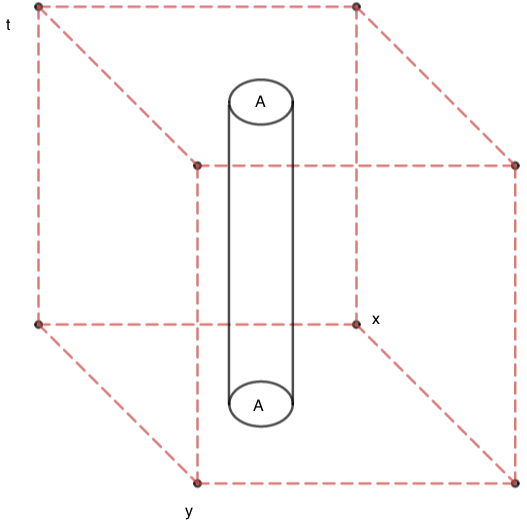
\includegraphics[scale=0.4]{10-3.png}
                    \caption{Drawing for Wangsness 10-3}
                \end{subfigure}
                \begin{subfigure}[b]{0.49\textwidth}
                    \centering
                    \captionsetup{type=figure}
                    \subimport{tikz/}{Wangsness_10_6}
                    \caption{Drawing for Wangsness 10-6}
                \end{subfigure}
            \end{figure}
            \subsubsection{Wangsness 10-17}
            Choose a spherical Gaussian surface outside the sphere concentric with the given sphere. $\int \mathbf{D}\cdot \mathbf{da} = Q_f$, so $D_o (4\pi r^2) = q$, and thus $\mathbf{D}_o = \frac{q}{4\pi r^2} \hat{\mathbf{r}}$. From $\mathbf{D} = \epsilon_0 \mathbf{E}+\mathbf{P}$, we have that $\mathbf{D}_o - \epsilon_0 \mathbf{E}_o = \mathbf{P}_o$. $\mathbf{E}_0 = \frac{q}{4\pi \epsilon_0 r^2}\hat{\mathbf{r}}$, and thus $\mathbf{P}_o = 0$. There is no dielectric outside of the sphere. Choosing a Gaussian surface inside of the sphere, we get $\int \mathbf{D}\cdot \mathbf{da} = Q_f$, for $D(4\pi r^2) = q$, and thus $\mathbf{D}_i = \frac{q}{4\pi r^2} \hat{\mathbf{r}}$. $\mathbf{E}_i = \frac{\mathbf{D}_i}{\epsilon} = \frac{\mathbf{D}_i}{\kappa_e \epsilon_0} = \frac{q}{4\pi \kappa_{e} \epsilon_0 r^2}\hat{\mathbf{r}}$. So $\mathbf{P}_i = \mathbf{D}_i - \epsilon_0 \mathbf{E}_i = (1-\frac{1}{\kappa_{e}}) \frac{q}{4\pi r^2} \hat{\mathbf{r}}$. Finally, $Q_b^{surface} = \int_{S} \sigma_{b} da' = \iint \mathbf{P}\cdot \hat{\mathbf{n}} da' = \int_{0}^{\pi} \int_{0}^{2\pi} \frac{\kappa_e-1}{\kappa_e} \frac{q}{4\pi} \sin(\theta) d\theta d\phi = \frac{\kappa_e-1}{\kappa_e} q$.
            \subsubsection{Wangsness 10-18}
            $\oint \mathbf{D} \cdot \mathbf{da} = q$. $\mathbf{D} = \frac{q}{4\pi r^2} \hat{\mathbf{r}}$ for all $r$ inside the cavity or in the dielectric. $\rho_b = 0$ since $\rho_f = 0$ in the dielectric. In the dielectric $\mathbf{E} = \frac{\mathbf{D}}{\epsilon} = \frac{\mathbf{D}}{\kappa_e \epsilon_0}$, so $\mathbf{E} = \frac{q}{4\pi \kappa_e \epsilon_0 r^2}\hat{\mathbf{r}}$. $\mathbf{P} = \mathbf{D}- \epsilon_0 \mathbf{E} = \frac{\kappa_e-1}{\kappa_e} \frac{q}{4\pi r^2} \hat{\mathbf{r}}$ at the surface of the cavity $r=a$. $\sigma_b = \mathbf{P}\cdot \hat{\mathbf{n}} = \frac{\kappa_e-1}{\kappa_e} \frac{q}{4\pi a^2} \hat{\mathbf{r}}\cdot (-\hat{\mathbf{r}}) = - \frac{\kappa_e-1}{\kappa_e} \frac{q}{4\pi a^2}$. $Q_b^{cavity} = \int \sigma da = - \frac{\kappa_e-1}{\kappa_e}q$.
            \subsubsection{Wangsness 10-25}
            $\kappa_e(x) = \alpha+\beta x$ (The dielectric constant varies linearly with $x$. $\alpha$ and $\beta$ are constants). Find $\mathbf{D}$ between the plates. $\int_{Gaussian Surface} \mathbf{D}\cdot \mathbf{da} = Q_f^{enc}$ (D is uniform between plates). $D\Delta a = Q_f^{enc}$, and thus $D = \frac{Q_f^{enc}}{\Delta a} = \sigma = \frac{Q}{A}$, where $Q$ is the total charge of the plate and $A$ is the area of the plate. $E = \frac{D}{\epsilon} = \frac{Q}{\kappa \epsilon_0 A} = \frac{Q}{\epsilon_0 A(\alpha + \beta x)}$. At $x=0$, $\kappa_e = \kappa_{e_1}$, so $\alpha+\beta(0) = \kappa_{e_1}$, and thus $\alpha = \kappa_{e_1}$. At $x=d$, $\kappa_{e} = \kappa_{e_2}$, and so $\beta = \frac{\kappa_{e_2}-\kappa_{e_1}}{d}$. The potential difference between the plates is $\Delta \phi = -\int_{-}^{+} \mathbf{E}\cdot \mathbf{d\ell} = \int_{+}^{-} Edx = \frac{Q}{\epsilon_0 A} \int_{0}^{d} \frac{dx}{\alpha+\beta x} = \frac{Q}{\epsilon A} \frac{1}{\beta} \ln(\alpha+\beta x)\big|_{0}^{d} = \frac{Q}{\epsilon_0 A\beta} \ln(\frac{\alpha+\beta d}{\alpha}) = \frac{Q}{\epsilon_0 A\beta} \ln(\frac{\kappa_{e_2}}{\kappa_{e_1}}) = \frac{Q}{C}$. Hence $C = \frac{\epsilon_0 A\beta}{\ln(\frac{\kappa_{e_2}}{\kappa_{e_1}})} = \frac{(\kappa_{e_2}-\kappa_{e_1})\epsilon_0 A}{d\ln(\frac{\kappa_{e_2}}{\kappa_{e_1}})}$
            \begin{figure}[H]
                \centering
                \captionsetup{type=figure}
                \begin{subfigure}[b]{0.49\textwidth}
                    \centering
                    \captionsetup{type=figure}
                    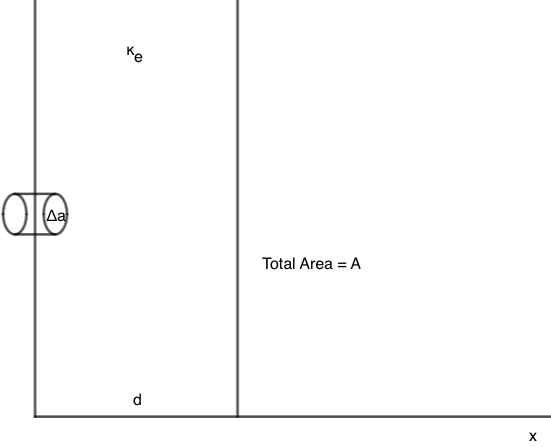
\includegraphics[width=\textwidth]{10-25.png}
                    \caption{Drawing for Wangsness 10-25}
                \end{subfigure}
                \begin{subfigure}[b]{0.49\textwidth}
                    \centering
                    \captionsetup{type=figure}
                    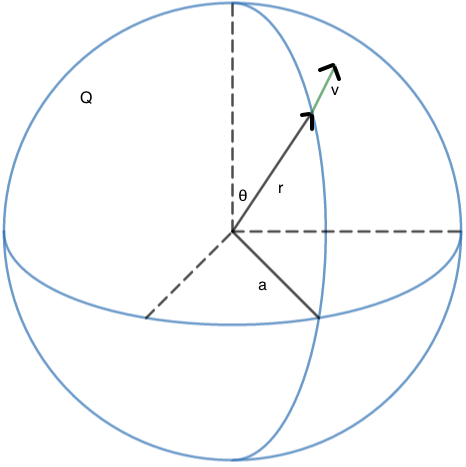
\includegraphics[width=\textwidth]{12-3.png}
                    \caption{Drawing for Wangsness 12-3}
              \end{subfigure}
            \end{figure}
            \subsubsection{Wangsness 10-27}
            $\kappa = \kappa_{e_1}$ for $a\leq \rho < \rho_0$, $\kappa = \kappa_{e_2}$ for $\rho_0 \leq \rho \leq b$. First get $D$ by assuming a charge per unit length $\lambda $on the inner cylinder and $-\lambda$ on the outer. $\int \mathbf{D}\cdot \mathbf{da} = Q_{f}^{enc} = D(2\pi \rho L) = \lambda L$. So $\mathbf{D} = \frac{\lambda}{2\pi \rho} \hat{\boldsymbol{\uprho}}$. $\Delta \phi = -\int_{-}^{+} \mathbf{E} \cdot \mathbf{d\ell} = \int_{a}^{b} \frac{\lambda}{2\pi \rho \epsilon}d\rho = \int_{a}^{\rho_0} \frac{\lambda}{2\pi \epsilon_0 \kappa_{e_1}\rho}d\rho + \int_{\rho_0}^{b} \frac{\lambda}{2\pi \epsilon_0 \kappa_{e_2}\rho}d\rho = \frac{\lambda}{2\pi \epsilon_0}\big[\frac{1}{\kappa_{e_1}}\ln(\frac{\rho_0}{a}) + \frac{1}{\kappa_{e_2}}\ln(\frac{b}{\rho_0})\big]$. From $\Delta \phi = \frac{Q}{C}$, and $Q=\lambda L$, we get $C = \frac{2\pi \epsilon_0 L}{\frac{1}{\kappa_{e_1}}\ln(\frac{\rho_0}{a}) + \frac{1}{\kappa_{e_2}}\ln(\frac{b}{\rho_0})}$
        \subsection{Homework XI}
            \subsubsection{Wangsness 12-3}
            $\mathbf{J} = \rho \mathbf{v}$. $\rho = \frac{Q}{\frac{4}{3}\pi a^3} = \frac{3q}{4\pi a^3}$. $\mathbf{u} = \mathbf{\omega}\times\mathbf{r} = \omega \hat{\mathbf{z}} \times r \hat{\mathbf{r}} = \omega r \sin(\theta) \hat{\boldsymbol{\upvarphi}}$. So, we have that $\mathbf{J} = \frac{3Q}{4\pi a^3} \omega r \sin(\theta) \hat{\boldsymbol{\upvarphi}}$. $\mathbf{da} = rdrd\theta \hat{\boldsymbol{\upvarphi}}$, so $I = \int \mathbf{J} \cdot \mathbf{da} = \frac{3Q \omega}{4\pi a^3} \int_{0}^{\pi} \int_{0}^{a} r^2\sin(\theta)drd\theta = \frac{Q\omega}{2\pi}$
            \subsubsection{Wangsness 13-4}
            We will calculate the force exerted by $C'$ on $C$. $\mathbf{F}_{C'\rightarrow C} = \frac{\mu_0}{4\pi} \oint_{C} \oint_{C'} \frac{I \mathbf{d\ell}\times (I' \mathbf{d\ell}'\times \hat{\mathbf{r}})}{R^2}$. We use the $BAC-CAB$ rule: $\mathbf{A}\times(\mathbf{B}\times \mathbf{C}) = \mathbf{B}(\mathbf{A}\cdot \mathbf{C}) - \mathbf{C}(\mathbf{A}\cdot \mathbf{B})$. We can rewrite the previous integral as  $\mathbf{F}_{C'\rightarrow C} = -\frac{\mu_0 II'}{4\pi} \oint_{C} \oint_{C'} \big[ \mathbf{d\ell}'\cdot(\mathbf{d\ell}\times \frac{\hat{\mathbf{r}}}{R^2}) - \frac{\hat{\mathbf{r}}}{R^2} \mathbf{d\ell}\cdot \mathbf{d\ell}\big]$. Recall that $\nabla(\frac{1}{R}) = \frac{\hat{\mathbf{r}}}{R^2}$. Using this, we have $\mathbf{F}_{C'\rightarrow C} = -\frac{\mu_0 II'}{4\pi} \oint_{C}\oint_{C'} \mathbf{d\ell'}\big[ \mathbf{d\ell}\cdot \nabla(\frac{1}{R})- \frac{\hat{\mathbf{r}}}{R^2} \mathbf{d\ell'} \cdot \mathbf{d\ell}\big]$. From the fundamental theorem of gradients, $\oint \nabla(f) \cdot \mathbf{d\ell} = 0$ for any function $f$. Thus $\oint \nabla(\frac{1}{R}) \cdot \mathbf{d\ell} = 0$. From this we have $\mathbf{F}_{C\rightarrow C'} = -\frac{\mu_0 II'}{4\pi} \oint_{C}\oint_{C'} \frac{\hat{\mathbf{r}}}{R^2} \mathbf{d\ell}'\cdot \mathbf{d\ell}$. We now compute this integral along all four paths of the problem. $\mathbf{d\ell}' = dz' \hat{\mathbf{z}}$ for all paths. Along path $I$, $\mathbf{r} = \hat{\mathbf{x}}d+\hat{\mathbf{z}}z$, $\mathbf{d\ell} = \hat{\mathbf{z}}dz$. Along path $III$, $\mathbf{r} = \hat{\mathbf{x}}(a+d)+\hat{\mathbf{z}}z$, $\mathbf{d\ell} = \hat{\mathbf{z}}dz$. Along paths $II$ and $IV$, $\mathbf{d\ell}\cdot \mathbf{d\ell}' = 0$. Piecing this together, $\mathbf{F}_{C\rightarrow C'} = -\frac{\mu_0 II'}{4\pi}\int_{0}^{b} \int_{-\infty}^{\infty} \frac{\hat{\mathbf{x}}d+\hat{\mathbf{z}}(z-z')}{\big(d^2+(z-z')^2\big)^{3/2}}dz'dz - \frac{\mu_0 II'}{4\pi} \int_{b}^{0} \int_{-\infty}^{\infty} \frac{\hat{\mathbf{x}}(d+a)+\hat{\mathbf{z}}(z-z')}{\big((d+a)^2+(z-z')^2\big)^{3/2}}dz'dz$. Making the substitution $t=z'-z$, we get an integral of the form $\int_{-\infty}^{\infty} \frac{t+z'}{(A+t^2)^{3/2}}dt$. This is an odd function that is integrated over symmetric bounds, and thus the integral is zero. The only part left is the $\hat{\mathbf{x}}$ contribution. Evaluating this integral, we get $\mathbf{F}_{C\rightarrow C'} = -\frac{\mu_0 II' ab}{2\pi d(a+d)}\hat{\mathbf{x}}$.
            \begin{figure}[htbp]
                \centering
                \captionsetup{type=figure}
                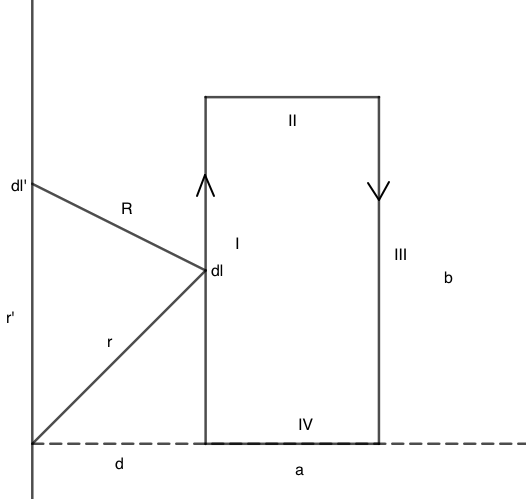
\includegraphics[scale=0.4]{13-4.png}
                \caption{Drawing for Wangsness 13-4}
            \end{figure}
            \subsubsection{Wangsness 14-7}
            $\mathbf{R} = \mathbf{r}-\mathbf{r}'$, where $\mathbf{r} = z\hat{\mathbf{z}}$ and $\mathbf{r}' = a\cos(\phi')\hat{\mathbf{x}}+a\sin(\phi')\hat{\mathbf{y}}$. We have $\boldsymbol{d\ell}' = ad\varphi' \hat{\boldsymbol{\upvarphi}}$. Putting this together, we have $\mathbf{R} = z\hat{\mathbf{z}} - a(\cos(\phi')\hat{\mathbf{x}}+\sin(\phi')\hat{\mathbf{y}})$. So:
            \begin{align*}
                \mathbf{B} &= \frac{\mu_0 I'}{4\pi}\int \frac{\boldsymbol{d\ell}\times \mathbf{R}}{R^3} = \frac{\mu_0I'}{4\pi} \int_{-\alpha}^{\alpha} \frac{ad\phi' \hat{\boldsymbol{\upvarphi}}\times (z\hat{\mathbf{z}}-a\cos(\phi')\hat{\mathbf{x}}-a\sin(\phi')\hat{\mathbf{y}})}{(z^2+a^2)^{3/2}}\\
                &= \frac{\mu_0 I'a}{4\pi(z^2+a^2)^{3/2}}\int_{-\alpha}^{\alpha} (-\sin(\phi')\hat{\mathbf{x}}+\cos(\phi')\hat{\mathbf{y}})\times (-a\cos(\phi')\hat{\mathbf{x}}-a\sin(\phi')\hat{\mathbf{y}}+z\hat{\mathbf{z}})d\phi'\\
                &= \frac{\mu_0 I'a}{4\pi (z^2+a^2)^{3/2}}\int_{-\alpha}^{\alpha} (z\cos(\phi')\hat{\mathbf{x}}+z\sin(\phi')\hat{\mathbf{y}}+a\hat{\mathbf{z}})d\phi'
            \end{align*}
            Sine is an odd function, and the limit is over a symmetric interval, and thus the $\hat{\mathbf{y}}$ component is zero. So we have:
            \begin{equation*}
                \mathbf{B} = \frac{\mu_0 I' a}{2\pi (z^2+a^2)^{3/2}}\big(z\sin(\alpha)\hat{\mathbf{x}}+a\alpha \hat{\mathbf{z}}\big)    
            \end{equation*}
            \subsubsection{Wangsness 14-15}
            The force on $q$ is given by $\mathbf{F} = q\mathbf{v}\times \mathbf{B}$. We first get $\mathbf{B}$ at $q$. $\mathbf{B} = \frac{\mu_0}{4\pi} \int \frac{I' d\ell' \times \hat{\mathbf{r}}}{R^2}$. For this problem, $\mathbf{R} = -\rho' \hat{\boldsymbol{\uprho}}$. We need only compute the integral along paths $I$ and $III$, for along $II$ and $IV$ we have that $\mathbf{d\ell}$ and $\mathbf{R}$ are parallel. So, we have $\mathbf{B} = \frac{\mu_0}{4\pi} \int_{0}^{\pi} \frac{I'(-ad\phi' \hat{\boldsymbol{\upvarphi}})\times (-a\hat{\boldsymbol{\uprho}})}{a^3}+ \frac{\mu_0}{4\pi} \int_{0}^{\pi} \frac{I'(bd\phi' \hat{\boldsymbol{\upvarphi}})\times (-b\hat{\boldsymbol{\uprho}})}{b^3} = \frac{\mu_0 I'}{4} \frac{b-a}{ab} \hat{\mathbf{z}}$. The force is $\mathbf{F} = qv\hat{\mathbf{y}} \times \frac{\mu_0 I}{4} \frac{b-a}{ab} \hat{\mathbf{z}} = \frac{qv\mu_0 I'}{4} \frac{b-a}{ab} \hat{\mathbf{x}}$
            \begin{figure}[htbp]
                \centering
                \captionsetup{type=figure}
                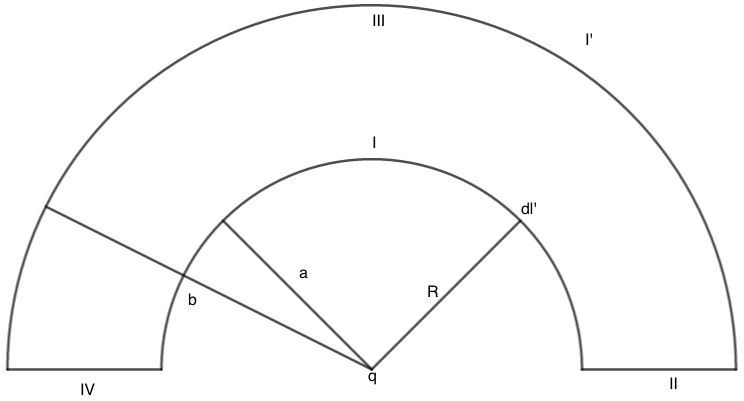
\includegraphics[scale=0.4]{14-15.png}
                \caption{Drawing for Wangsness 14-15}
            \end{figure}
        \subsection{Homework XII}
            \subsubsection{Wangsness 15-7}
            For $\rho\leq a$, path $(1)$ has $\oint \mathbf{B}\cdot \mathbf{d\ell}= \mu_0 I_{enc}$, where $I_{enc} = I\frac{\rho^2}{a^2}$. So $\mathbf{B} = \frac{\mu_0 I\rho}{2\pi a^2} \hat{\boldsymbol{\upvarphi}}$. For $a\leq \rho \leq b$, $I_{enc} = I$. So $B = \frac{\mu_0 I}{2\pi \rho} \hat{\boldsymbol{\upvarphi}}$. For $b\leq \rho \leq c$, $I_{enc} = I =I\frac{\rho^2-b^2}{c^2-b^2} = I\frac{c^2-\rho^2}{c^2-b^2}$. So $\mathbf{B} = \frac{\mu_0 I}{2\pi \rho} \frac{c^2-\rho^2}{c^2-b^2}\hat{\boldsymbol{\upvarphi}}$. Finally, or $\rho \geq c$, $I_{enc} = 0$, so $\mathbf{B} = 0$.
            \begin{figure}[htbp]
                \centering
                \captionsetup{type=figure}
                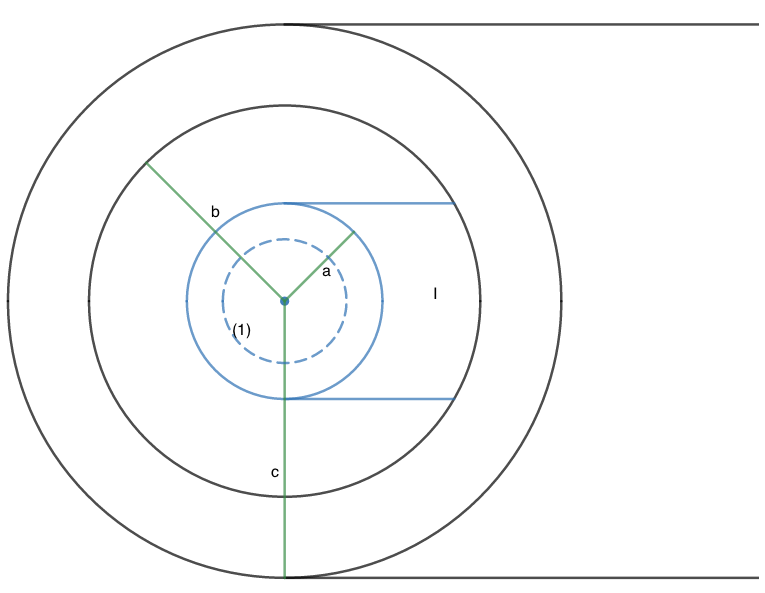
\includegraphics[scale=0.4]{15-7.png}
                \caption{Drawing for Wangsness 15-7}
            \end{figure}
            \subsubsection{Wangsness 15-8}
            \begin{equation*}
                \mathbf{B}=
                    \begin{cases}
                        0,&\rho<a\\
                        \frac{\mu_0 I}{2\pi \rho}
                        \frac{\rho^2-a^2}{b^2-a^2}
                        \hat{\boldsymbol{\upvarphi}},
                        &a<\rho<b\\
                        \frac{\mu_0 I}{2\pi \rho} \hat{\boldsymbol{\upvarphi}},
                        &\rho>b
                    \end{cases}    
            \end{equation*}
            By definition, $\mu_0 \mathbf{J} = \nabla \times \mathbf{B}$. So:
            \begin{equation*}
                \mathbf{J} = \begin{cases} 0, & \rho<a\\ \frac{I}{\pi(b^2-a^2)}, & a<\rho < b\\ 0, & \rho>b \end{cases}    
            \end{equation*}
            The current $I$ i distributed uniformly over the volume between two coaxial cylinders of inner radius $a$ and outer radius $b$ in the direction of the cylinder axis.
            \subsubsection{Wangsness 16-10}
            The field point is on the $z-$axis. $\mathbf{r} = z\hat{\mathbf{z}}$, $\mathbf{r}' =  a\cos(\phi')\hat{\mathbf{x}}+a\sin(\phi')\hat{\mathbf{y}}$. $\mathbf{d\ell}' = \mathbf{dr}' = ad\phi' \hat{\boldsymbol{\upvarphi}} = ad\phi' (-\sin(\phi')\hat{\mathbf{x}}+\cos(\phi')\hat{\mathbf{y}})$. $\mathbf{A} = \frac{\mu_0 I'}{4\pi} \int \frac{\mathbf{d\ell}'}{R} = \frac{\mu_0 I'}{4\pi} \frac{a}{\sqrt{a^2+z^2}}\int_{-\alpha}^{\alpha} (-\sin(\phi')\hat{\mathbf{x}}+\cos(\phi')\hat{\mathbf{y}})d\phi' = \frac{\mu_0 I'a}{2\pi \sqrt{a^2+z^2}}\sin(\alpha)\hat{\mathbf{y}}$. To find $\mathbf{B}$ from $\mathbf{A}$, we need to evaluate $\nabla \times \mathbf{A}$. We don't know about $\mathbf{A}$ for a general point, and thus we can't evaluate the $x$ and $y$ derivatives.
        \subsection{Homework XIII}
            \subsubsection{Wangsness 17-3}
            The $\mathbf{B}$ field associated with $I$ is $\mathbf{B} = \frac{\mu_0 I}{2\pi \rho} \hat{\boldsymbol{\upvarphi}}$. In the plane of the paper, $\phi$ is into the paper. $\Phi = \int \mathbf{B}\cdot \mathbf{da} = \int \frac{\mu_0 I}{2\pi \rho} \cdot b d\rho \hat{\boldsymbol{\upvarphi}} = \frac{\mu_0Ib}{2\pi} \int_{d}^{d+a} \frac{d\rho}{\rho}= \frac{\mu_0 Ib}{2\pi} \ln(\frac{d+a}{d}) = \frac{\mu_0 bI_0 e^{-\lambda t}}{2\pi} \ln(\frac{d+a}{d}) = \frac{\mu_0 I_0 \lambda b}{2\pi} \ln(\frac{d+a}{d})e^{-\lambda t}$. The induced current is clockwise around the loop to produce a field which goes into the paper to counteract the decreasing $\mathbf{B}$ due to $I_0$.
            \subsubsection{Wangsness 17-4}
            The $\mathbf{B}-$field at distance $\rho$ from the wire at points in the plane of the paper is $\mathbf{B} = \frac{\mu_0 I}{2\pi \rho} \hat{\mathbf{y}}$. The flux of $\mathbf{B}$ through the loop is $\Phi = \int \mathbf{B}\cdot \mathbf{da} = \iint \frac{\mu_0 I}{2\pi \rho}\rho d\theta d\rho$. We have $\rho = b+r\cos(\theta)$. So $\Phi = \frac{\mu_0 I}{2\pi} \int_{0}^{a} \int_{0}^{2\pi} \frac{r d\theta dr}{b+r\cos(\theta)} = \frac{\mu_0 I}{2\pi} \int_{0}^{a} \frac{2r}{\sqrt{b^2-r^2}}\tan^{-1}\big[\frac{\sqrt{b^2-r^2}\tan(\theta/2)}{b+r}\big]_{0}^{2\pi} \Rightarrow \tan^{-1}\big[\frac{\sqrt{b^2-r^2}}{b+r}\tan(\pi)\big] - \tan^{-1}\big[ \frac{\sqrt{b^2-r^2}}{b+r}\tan(0)\big]$. So $\Phi = \mu_0 I\big[b-\sqrt{b^2-a^2}\big]$. The loop moves with constant speed $v$ along the $x-$axis away from the current $I$, $v = \frac{db}{dt}$. So $\xi = -\frac{d\Phi}{dt} = -\mu_0 I \frac{d}{dt}\big[b-\sqrt{b^2-a^2}\big] = -\mu_0 I\big[ v-\frac{bv}{\sqrt{b^2-a^2}}\big] = \mu_0 NIv\big[ \frac{b}{\sqrt{b^2-a^2}}-1\big]$. The current will be clockwise trying to increase the flux which is decreasing due to motion away from the wire.
            \begin{figure}[htbp]
                \centering
                \captionsetup{type=figure}
                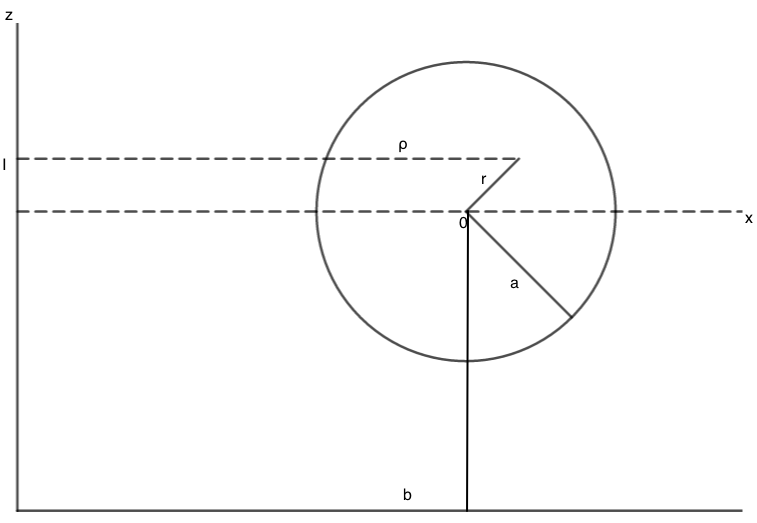
\includegraphics[scale=0.4]{17-4.png}
                \caption[Drawing for Wangsness 17-4]{Drawing for Wangness 17-4}
            \end{figure}
            \subsubsection{Wangsness 17-19}
            $\Phi_{12} = IM_{12}$. The flux due to $1$ through $2$ is $\Phi_{12} = \int \mathbf{B}_1 \cdot \mathbf{da}_2$. $\mathbf{B}_1 = \frac{\mu_0 I}{2\pi} \big( \frac{1}{\rho+d}- \frac{1}{\rho+d+D}\big)$. So we have that $\Phi_{12} = \int_{0}^{a} \frac{\mu_0 I}{2\pi} \big(\frac{1}{\rho+d}- \frac{1}{\rho+d+D}\big) bd\rho = \frac{\mu_0 Ib}{2\pi}\big[ \ln(\frac{a+d}{a+d+D}) - \ln(\frac{d}{d+D})\big]$. Thus, we have $M = \frac{\mu_0 b}{2\pi} \ln\big(\frac{a+d}{d}\big)$
            \subsubsection{Wangsness 17-20}
            The field inside the toroid is $\mathbf{B} = \frac{\mu_0 NI}{2\pi \rho} \hat{\boldsymbol{\upvarphi}}$. The flux through a single turn is $\Phi^1 = \frac{\mu_0 NI}{2\pi} \int_{0}^{a} \int_{0}^{2\pi} \frac{r}{b+r\cos(\theta)}d\theta dr$. We've done this integral before, and we get $\Phi^1= \mu_0 NI\big[b-\sqrt{b^2-r^2}\big]$. $\Phi = N\Phi^1$. $L = \frac{\Phi}{I} = \frac{\mu_0 N^2 I}{I} \big[b-\sqrt{b^2-r^2}\big] = \mu_0 N^2 \big[b-\sqrt{b^2-r^2}\big]$
    \section{Exams}
        \subsection{Exam I}
        \subsubsection{Question I}
        Give the vector field field $\mathbf{A} = c\hat{\boldsymbol{\uptheta}}$, where $c$ is a constant, find $\nabla \times \mathbf{A}$. Is this a conservative vector field? Explain.
        \subsubsection{Question II}
        Verify the Divergence Theorem for $\mathbf{A}$ given in problem 1 in spherical coordinates for a hemisphere of radius $a_0$ resting on the $xy-plane$ with the center of the flat base of the hemisphere at the origin and the symmetry axis of the hemisphere along the positive $z-axis$.
        \subsubsection{Question III}
        A semicircular charged line of radius $a$ carries uniform linear charge density $\lambda$. It has the equation $x^2+y^2 = a^2$, $x\geq 0$, $z=0$. That is, the half circle resting on the $xy-plane$ of radius $a$. Find the electring field at a point $P$ on the $z$ axis a distance $z$ from the origin.
        \subsection{Exam II}
        \subsubsection{Question I}
        A conducting sphere of radius $a$, centered at the origin carries charge $Q_1$. This sphere is surrounded by a hollow concentric conducting spherical shell of inner radius $b$ and outer radius $c$ with $a<b<c$. The outer hollow conducting shell caries a total charge $Q_2$. 
        \begin{enumerate}
            \item What is the electric field everywhere?
            \item What is the potential everywhere, assuming $\underset{r\rightarrow \infty} \lim \phi(r) = 0$?
            \item How much charge is on the inner and outer surfaces of the conducting shell at $r=b$ and $r=c$?
        \end{enumerate}
        \subsubsection{Question II}
        The outer conductor of problem I is now grounded.
        \begin{enumerate}
            \item What is the electric field everywhere?
            \item What is the potential everywhere?
            \item How much charge is on the surfaces at $r=b$ and $r=c$?
            \item What is the capacitance of the system of conductors?
            \item Calculate the electrostatic potential energy of the configuration assuming the energy resides in the charges.
            \item Calculate the electrostatic potential energy of the configuration assuming the energy resides in the electric field.
        \end{enumerate}
        \subsubsection{Question III}
        A semicircular arc of radius $a$ in the $y-z$ plane with center on the $y-axis$ at the origin and the top of the arc on the positive $y-axis$ carries linear charge density $\lambda = \lambda_0 \cos(\theta')$, where $\lambda_0$ is constant and $\theta'$ is measured with respected to the positive $z-axis$.
        \begin{enumerate}
            \item What is the electric monopole moment of this distribution?
            \item What is the electric dipole moment of this distribution?
            \item What is the electric potential at a distance $r$ from the origin for this distribution where $r>a$, accurate to order $\frac{1}{r^2}$?
        \end{enumerate}
        \subsection{Exam III}
        \subsubsection{Question I}
        The electric field in a spherical region of space of radius $a$ is given by $\mathbf{E} = E_0 \frac{r^2}{a^2}\hat{\mathbf{r}}$ for $r< a$, where $E_0$ is a constant. This region is surrounded concentrically by a grounded conducting spherical shell of inner radius $b$ and outer radius $c$ with $a<b<c$. There is no charge in the region $a<r<b$. 
        \begin{enumerate}
            \item What is the electric charge density in the region $r<a$?
            \item Wher is the electric field in the region $a<r<b$?
            \item How much charge is on the surfaces at $r=b$ and $r=c$?
            \item What is the electric field for $r>c$?
            \item What is the electric potential $\phi$ at $r=0$ assuming that ground potential is $\phi = 0$.
        \end{enumerate}
        \subsubsection{Question II}
        A capacitor $C_{1}$ is charged to a potential difference $\Delta \phi$ between its plates. A second capacitor $C_{2}$ is uncharged. One plate of $C_2$ is now connected to a plate of $C_1$ by a conductor of negligible capacitance, the remaining plates are similarly connected. 
        \begin{enumerate}
            \item For the resultant equilibrium state, find the charge on each capacitor and the potential difference $\Delta \phi$ between their respective plates.
            \item Compare the energy stored in capacitor $C_1$ before connecting it to $C_2$, to the energy of the combination after connected them. Are these energies the same? If not, which is larger and where did any additional energy come from, or where did any lost energy go?
        \end{enumerate}
        \subsubsection{Question III}
        Find the electric dipole moment of an hourglass configuration of charge consisting of two identical right circular cones of radius $a$ and height $a$ with symmetry axes aligned apex to apex along the $z-$axis with the apexes touching at the origin. The top cone has charge density $\sigma_0$ on its surface, and the bottom cone has charge density $-\sigma_0$ on its surface.
        \subsection{Practice Final Exam}
        \subsubsection{Problem I}
        The electric field in a region of space is given in spherical coordinates as $\mathbf{E} = cr\hat{\mathbf{r}}$, where $c$ is constant. 
        \begin{enumerate}
            \item Find the charge density at a point $(r,\theta,\phi)$
            \item Find the total charge inside a sphere of radius $a$ centered at the origin.
        \end{enumerate}
        \subsubsection{Problem II}
        A battery is used to charge an ideal parallel plate capacitor to a potential difference $\Delta \phi = V_0$. The battery is then disconnected. The separation between the plates is now increasing from $d$ to $\alpha d$, where $\alpha >1$. The area of the plates is $A$.
        \begin{enumerate}
            \item What is the ratio of the new energy to the original energy>
            \item Is the energy increases or decreased?
            \item Where does this energy come from or go to?
            \item Compute the change in energy $\Delta U_e$ expressing your answer in terms of the given quantities $V_0,d,A,\alpha$ and fundamental constants.
        \end{enumerate}
        \subsubsection{Problem III}
        A dielectric sphere of radius $a$ and permittivity $\varepsilon$ contains a free charge density. $\rho_f = cr$, where $c$ is a constant. The sphere is centered at the origin. Find the electric potential at the center of the sphere assuming that the potential is zero at an infinite distance from the center.
        \subsubsection{Problem IV}
        A thick slab extending from $z=-a$ to $z=a$ carries a uniform vlume current density $\mathbf{J} = J_0 \hat{\mathbf{x}}$. The slab is infinite in the $xy-$plane. Find the magnetic field $B$ as a function of $z$ inside and outside the slab. Plot $B$ as a function of $z$ for $-b<z<b$ where $b>a$.
        \subsubsection{Problem V}
        An ideal long solenoid of radius $a$, carrying $n$ turns per unit length, is looped by a wire with resistance $R$. 
        \begin{enumerate}
            \item If the current in the solenoid is increasing at a constant rate $\frac{dI}{dt} = k$, what current flows in the lopp, and which way (Left or right) does it pass through the resistor?
            \item If the current $I$ in the solenoid is constant but the solenoid is pulled out of the loop and reinserted in the opposite direction, what total charge passes through the resistor?
        \end{enumerate}
        \subsection{Final Exam}
        \subsubsection{Problem I}
        \begin{enumerate}
            \item Write down Maxwell's Equations in differential form.
            \item Convert them to integral form and show derivations.
            \item Name each equation.
        \end{enumerate}
        \begin{proof}[Solution]
        \
        \begin{enumerate}
        \item Gauss' Law: $\nabla \cdot \mathbf{E} = \frac{\rho}{\epsilon_0}\Rightarrow\frac{Q_{encl}}{\epsilon_0}=\iiint_{V} \frac{\rho}{\epsilon_0}d\tau=\iiint_{V} \big(\nabla \cdot \mathbf{E}\big) d\tau = \oiint_{\partial V} \mathbf{E}\cdot \mathbf{da}$
        \item Faraday's Law: $\nabla \times \mathbf{E} = -\frac{\partial \mathbf{B}}{\partial t}\Rightarrow-\frac{d \Phi_{B}}{dt} = \iint_{S} -\frac{\partial \mathbf{B}}{\partial t}da = \iint_{S} \big(\nabla \times \mathbf{E}\big)da = \oint_{\partial S}\mathbf{E}\cdot \mathbf{d\ell}$
        \item Gauss' Law of Magnetism: $\nabla \cdot \mathbf{B} = 0\Rightarrow 0 = \iiint_{V} \big(\nabla \cdot\mathbf{B}\big)d\tau = \oiint_{\partial V} \mathbf{B}\cdot \mathbf{da}$
        \item Ampere's Law: $\nabla \times \mathbf{B} = \mu_0 \mathbf{J} + \mu_0 \epsilon_0 \frac{\partial \mathbf{E}}{\partial t}\Rightarrow\mu_0 I_{encl}+ \mu_0 \epsilon_0 \frac{d\Phi_{E}}{dt} = \iint_{S}\big(\mu_0 \mathbf{J} + \mu_0 \epsilon_0 \frac{\partial \mathbf{E}}{\partial t}\big)da = \iint_{S}\big(\nabla \times \mathbf{B}\big)da = \oint_{\partial S}\mathbf{B}\cdot \mathbf{d\ell}$
        \end{enumerate}
        \end{proof}
        \subsubsection{Problem II}
        A conduction sphere of radius $a$ carries a charge $Q_{1}$. It is surrounded by a conducting spherical shell of inner radius $b$ and outer radius $c$ with $a<b<c$. The charge on the conducting shell is $Q_{2}$. The region between the conductors $a<r<b$ is filled with linear isotropic dielectric of permittivity $\varepsilon$. Find the following in the regions $r<a.a<r<b.b<r.b<r<c.c<r$:
        \begin{enumerate}
            \item The electric displacement $\mathbf{D}$
            \item The electric field $\mathbf{E}$
            \item The polarization vector $\mathbf{P}$
            \item Find the free charge on the conductors at $r=a,b,c$.
            \item The bound volume charge in the dielectric.
            \item The bound surface charge density at the inner and outer surfaces of the dielectric.
            \item The electric potential at the origin assuming the potential is zero as $r$ goes to infinity.
        \end{enumerate}
        \begin{proof}[Solution]
        \
        \begin{enumerate}
        \begin{multicols}{2}
            \item $\mathbf{D}=\begin{cases}\mathbf{0}&r<a\\ \frac{Q_{1}}{4\pi r^{2}} &a<r<b\\\mathbf{0} & b<r<c\\ \frac{Q_{1}+Q_{2}}{4\pi r^{2}} & c<r \end{cases}$
            \item $\mathbf{E}=\begin{cases}\mathbf{0}&r<a\\ \frac{Q_{1}}{4\pi\epsilon_{0} r^{2}} & a<r<b\\ \mathbf{0} & b<r<c\\ \frac{Q_{1}+Q_{2}}{4\pi\epsilon_{0}r^{2}} & c<r\end{cases}$
            \item $\mathbf{P}=\begin{cases}\mathbf{0}&r<a\\ \frac{Q_{1}}{4\pi r^{2}}(1-\frac{\epsilon_{0}}{\varepsilon}) & a<r<b\\ \mathbf{0} & b<r<c\\ \mathbf{0} & c<r \end{cases}$
            \item $Q = \begin{cases} Q_1 & r=a\\ -Q_1 & r=b\\ Q_1+Q_2 & r=c\end{cases}$
        \end{multicols}
        \begin{multicols}{2}
            \item $\rho_b = \nabla \cdot \mathbf{P}$, $\rho_b = 0$.
            \item $\sigma_{b,a}=-\frac{Q_1}{4\pi a^2}\big(1-\frac{\epsilon_0}{\varepsilon}\big)$, $\sigma_{b,b}=\frac{Q_1}{4\pi b^2}\big(1-\frac{\epsilon_0}{\varepsilon}\big)$.
            \end{multicols}
            \item $\phi = -\int_{0}^{\infty}\mathbf{E}\cdot \mathbf{d\ell} = \int_{c}^{\infty} \mathbf{E}\cdot \mathbf{d\ell}+\int_{b}^{c}\mathbf{E}\cdot \mathbf{d\ell}+\int_{a}^{b}\mathbf{E}\cdot \mathbf{d\ell} + \int_{0}^{a} \mathbf{E}\cdot \mathbf{d\ell} = \frac{Q_1+Q_2}{4\pi \epsilon_0 c}+\frac{Q_1}{4\pi \epsilon_0 a}-\frac{Q_1}{4\pi \epsilon_0 b}$.
        \end{enumerate}
        \end{proof}
        \subsubsection{Problem III}
        A sphere of radius $a$ carries charge density $\rho = \rho_0(r/a)$, where $\rho_0$ is a constant. Find the work done to assemble the charge distribution.
        \begin{proof}[Solution]
        We find $\mathbf{E}$ inside and outside using Gauss' law.
        \begin{equation*}
        \oiint_{S} \mathbf{E}\cdot \mathbf{da} = \frac{Q_{encl}}{\epsilon_0} = \int_{0}^{r}\int_{0}^{\pi} \int_{0}^{2\pi} \rho_0 \frac{r}{a}r^2\sin(\theta)d\varphi d\theta dr = \frac{4\pi \rho_0}{a \epsilon_0}\frac{r^4}{4} = E(4\pi r^2).
        \end{equation*}
        So $\mathbf{E} = \frac{\rho_0 r^2}{4a\epsilon_0}\hat{\mathbf{r}}$. Outside we have $\oiint_{S} \mathbf{E}\cdot \mathbf{da} = \int_{0}^{2\pi}\int_{0}^{\pi} \int_{0}^{a} \rho \frac{r}{a}r^2 \sin(\theta) dr d\theta d\varphi$, so $\mathbf{E} = \frac{\rho_0 a^3}{4r^2 \epsilon_0}\hat{\mathbf{r}}$. The work is
        \begin{align*}
        \frac{\epsilon_0}{2}\int_{All\ Space}E^2 d\tau &= \frac{\epsilon_0}{2}\int_{0}^{2\pi}\int_{0}^{\pi}\int_{0}^{\infty} E^2 r^2\sin(\theta) drd\theta d\varphi\\
        &= \int_{0}^{2\pi}\int_{0}^{\pi}\int_{0}^{a} E^2r^2\sin(\theta)dr d\theta d\varphi + \int_{0}^{2\pi}\int_{0}^{\pi}\int_{a}^{\infty} E^2r^2\sin(\theta)drd\theta d\varphi\\
        &= \frac{\pi \rho_0^2 a^5}{7\epsilon_0}
        \end{align*}
        So $\mathbf{E} = \frac{\rho_0 r^2}{4a\epsilon_0}\hat{\mathbf{r}}$
        \end{proof}
        \subsubsection{Problem IV}
        \begin{enumerate}
            \item Could the vector field $\mathbf{F} = ax\hat{\mathbf{x}}+by\hat{\mathbf{y}}+cz\hat{\mathbf{z}}$ be a possible magnetic field, where $a+b+c\ne 0$? Explain why or why not.
            \item An electric field is given by $\mathbf{E} = ax\hat{\mathbf{y}}$, where $a$ is a constant. Is this a conservative field? Explain why or why not.
            \item Find the possible magnetic field $\mathbf{B}$ associated to $\mathbf{E}$. 
        \end{enumerate}
        \begin{proof}[Solution]
        \
        \begin{enumerate}
            \item No, for $\nabla \cdot \mathbf{F} = a+b+c \ne 0$, and therefore $\mathbf{F}$ cannot be a magnetic field.
            \item No, for $\nabla \times \mathbf{E} = a\hat{\mathbf{z}} \ne 0$, and thus $\mathbf{E}$ is not a conservative field.
            \item $\nabla \times \mathbf{E} = -\frac{\partial \mathbf{B}}{\partial t} = a\hat{\mathbf{z}}$, so $\mathbf{B} = -at\hat{\mathbf{z}}+\mathbf{B}_0$, where $\mathbf{B}_0$ is some constant vector. Here $\mathbf{B}$ is increasing with time in the $-z$ direction.
        \end{enumerate}
        \end{proof}
        \subsubsection{Problem V}
        Two infinitely long coaxial cylindrical infinitesimally
        thin conducting shells concentric with the $z-$axis carry
        oppositely directed currents of equal magnitude in the $+$
        and $-$ $z-$directions. The radius of the inner shell is $a$
        and that of the outer shell is $b$. What is the self-inductance
        of a length $\ell$ of this system?
        \begin{proof}[Solution]
        The flux carried by the inner shell cuts through the area of a rectangle of lenght $\ell$ and width $b-a$. So $\Phi = \int \mathbf{B}\cdot \mathbf{da} = \int_{a}^{b} \frac{\mu_0 I}{2\pi \rho}\ell d\rho = \frac{\mu_0 I\ell}{2\pi}\ln\big(\frac{b}{a}\big)$. So, $L = \frac{\Phi}{I} = \frac{\mu_0 \ell}{2\pi}\ln\big(\frac{b}{a}\big)$.
        \end{proof}
\end{document}